\chapter{Conservación de Suelos y Aguas}
\section{Introducción}
Al estudiar el sistema suelo-agua, entendiendo sus principales característica físicas mediante su conceptualización utilizando modelos para relacionarlas con los procesos erosivos del suelo, además enlistando los demás objetivos:
\begin{itemize}
    \item Estudiar la mecánica del proceso erosivo y sus agentes causales mediante su conceptualización, para ver sus implicaciones en la producción agrícola, el medio ambiente y su efecto sobre la sociedad.
    \item Estimar y predecir la erosión del suelo mediante la aplicación de métodos y modelos, para poder proponer técnicas de conservación y manejo de las tierras y escurrimientos superficiales.
    \item Cuando se refiere a las tierras, es un concepto que incluye a los suelos, pero también a la vegetación, agrometeoros e incluso el uso humano del lugar.
    \item Estudiar y analizar los diferentes tipos de obras y prácticas mecánicas, vegetativas y agronómicas utilizadas para la conservación y manejo del suelo y el agua, mediante su conceptualización, considerando los criterios de aplicación, funcionamiento, diseño, trazo, construcción, para su implementación en los sitios necesarios.
\end{itemize}
\subsection{Panorama mundial de los recursos naturales principales}

\begin{definition}[Recursos naturales]
Son aquellos que existen en el ambiente sin ninguna acción humana, algunos de ellos son esenciales para la sobrevivencia humana, mientras que otros satisfacen necesidades de la sociedad

Las \textbf{Renovables} se pueden utilizar una y otra vez, siempre y cuando el hombre cuide su regeneración

Las \textbf{No renovables} al ser utilizados no pueden ser regenerados \footnote{Para formar 1 centímetro de suelo, se necesitan miles de años}
\end{definition}

¿Por qué ah adquirido tanta importancia su manejo? su manejo tiene relación con problemas ambientales pues impacta:
\begin{itemize}
    \item Calentamiento global
    \item Destrucción de la capa de ozono
    \item Pérdida de la biodiversidad
    \item Pérdida de tierras cultivables
    \item Contaminación del aire, agua y suelo
\end{itemize}

El procedimiento a seguir en cualquier sistema:
\begin{enumerate}
    \item Definir el problema
    \item Actividades del hombre que originan u originaron el problema
    \item Metas a alcanzar con relación al problema
    \item Actividades a realizar para alcanzar las metas
\end{enumerate}

Ejemplo para el suelo
\begin{enumerate}
    \item Pérdida de la fertilidad del suelo
    \item No propiciar la pérdida de la fertilidad del suelo
    \item Manejo inadecuado
    \item Utilizar técnicas de manejo que eleven o mantengan la fertilidad del suelo
\end{enumerate}
Ejemplo para el agua
\begin{enumerate}
    \item Pérdida de la recarga de acuíferos
    \item Urbanización en zonas de recarga
    \item No propiciar la pérdida de la capacidad de recarga
    \item Identificar zonas de recarga y legislar
\end{enumerate}
Ejemplo para la vegetación
\begin{enumerate}
    \item Pérdida de la cobertura vegetal
    \item Deforestación
    \item No propiciar la pérdida de la cobertura vegetal
    \item Proponer un plan de manejo forestal y legislar
\end{enumerate}
El principal problema es la escasez, gracias a la explosión demográfica, contaminación, deforestación y cambio climático

¿Cuál es el principal problema del suelo?

\begin{remark}
    La degradación del suelo se divide en:
    \begin{enumerate}
        \item Física
        \begin{enumerate}
            \item Endurecimiento
            \item Erosión y desertificación \begin{enumerate}
                \item Erosión hídrica
                \item Erosión eólica
            \end{enumerate}
        \end{enumerate}
        \item Química \begin{enumerate}
            \item Disminución de la fertilidad
            \item Desequilibrio elemental \begin{enumerate}
                \item Salsodificación 
                \item Componentes tóxicos 
                \item Acidificación
            \end{enumerate}
        \end{enumerate}
        \item Biológica \begin{enumerate}
            \item Producción de micro y macro fauna
            \item Pérdida de la materia orgánica
        \end{enumerate}
    \end{enumerate}
\end{remark}
\begin{table}[h!]
    \centering
    \begin{tabular}{@{}cc@{}}
    \toprule
    Degradación & Porcentaje de incidencia \\ \midrule
    Hídrica     & 56                       \\
    Eólica      & 28                       \\
    Química     & 12                       \\
    Física      & 4                        \\ \bottomrule
    \end{tabular}
    \caption{Principales tipos de degradación en el mundi}
    \label{tabcsa1}
\end{table}

\begin{table}[h!]
    \centering
    \begin{tabular}{@{}ll@{}}
    Grad     & \%    \\
    Extrema  & 6.79  \\
    Fuerte   & 5.79  \\
    Moderada & 26.37 \\
    Leve     & 37.06
    \end{tabular}
    \caption{En México el 76\% por ciento de la superficie tiene algún grado de erosión hídrica}
    \label{tabcsa2}
\end{table}
\begin{figure}[h!]
\centering
  \includegraphics[width=0.8\textwidth]{csa1.png}
  \caption{Tipos de vegetación en México}
  \label{csa1}
\end{figure}
\begin{figure}[h!]
\centering
  \includegraphics[width=0.5\textwidth]{csa2.jpg}
  \caption{Tipos de Clima en México}
  \label{csa2}
\end{figure}
\begin{figure}[h!]
\centering
  \includegraphics[width=0.5\textwidth]{csa3.jpg}
  \caption{Precipitación en México}
  \label{csa3}
\end{figure}

México se encuentran 26 de los 32 grupos de suelos reconocidos por le sistema internacional base de referencia mundial del Recurso suelo.

El territorio nacional está cubierto en un 81.7\% por seis grupos de suelos:
\begin{itemize}
    \item Leptosol (28.3\%)
    \item Regosol (13.7\%)
    \item Phaeozem (11.7\%) %Disque el mejor
    \item Calcisol (10.4\%)
    \item Luvisol (9.0\%) %Disque el mejor
    \item Vertisol (8.6\%) %Disque el mejor
\end{itemize}
El territorio restante lo cubren los otros 20 grupos de suelos reconocidos, la mayor parte del territorio (52.4\%) está cubierto por tres grupos de suelos someros y poco desarrollados lo que dificulta su aprovechamiento agrícola y aumentan su vulnerabilidad.
\subsubsection{¿Por qué aparece la erosión antrópica?}

Uno de los acontecimientos más importantes en la historia humana, ha sido el cambio de una economía sustentada en la caza y recolección de plantas a una basada en la agricultura.

Este cambio ocurrió de manera independiente en por lo menos seis regiones del mundo, entre los años 11,000 y 5,000 A.C. en áreas tropicales y subtropicales con alta biodiversidad; donde grupos recolectores y cazadores iniciaron la domesticación de plantas y animales

La erosión acelerada es tan antigua como  la agricultura, Se remonta a las antiguas civilizaciones en Mesopotamia, el colapso de las grandes civilizaciones antiguas a lo largo del Tigris - Éufrates ilustra las consecuencias de la degradación irreversible de las tierras.

\subsubsection{¿Por qué debemos conservar el suelo?}
Es un recurso fundamental y básico, los seres humanos no pueden sobrevivir sin tierra porque es la base de toda la vida terrestre. Es un recurso vital que sostiene la seguridad alimentaria y la calidad ambiental, ambas esenciales para la existencia humana; los suelos del mundo se manejan para:
\begin{itemize}
    \item Satisfacer la creciente demanda de almacenamientos
    \item Filtrar el aire
    \item Purificar el agua 
    \item Almacenar carbono
    \item Compensar las emisiones antropogénicas de $CO_2$
\end{itemize}
\begin{table}[h!]
    \centering
    \begin{tabular}{@{}cccc@{}}
    \toprule
    \begin{tabular}[c]{@{}c@{}}Seguridad alimentaria\\ biodiversidad y urbanización\end{tabular} &
      Calidad del agua &
      \begin{tabular}[c]{@{}c@{}}Impacto global y\\ cambio climático\end{tabular} &
      \begin{tabular}[c]{@{}c@{}}Producción de\\ alimento y\\ biocombustibles\end{tabular} \\ \midrule
    Alimentos                & Filtro de contaminantes & \begin{tabular}[c]{@{}c@{}}Sumideros de $CO_2$\\ y $CH_3$\end{tabular} & Pastos|  \\
    Fibras                   & Purifación del agua     & Captura de carbomo                                                     & Cultivos \\
    Alojamiento &
      \begin{tabular}[c]{@{}c@{}}Retención de\\ sedimentos y químicos\end{tabular} &
      \begin{tabular}[c]{@{}c@{}}Reducción de la\\ nitrificación\end{tabular} &
       \\
    Recreación &
      \begin{tabular}[c]{@{}c@{}}Amortiguamiento y\\ transformación de\\ químicos\end{tabular} &
      \begin{tabular}[c]{@{}c@{}}Depósito y entierro de\\ sedimentos ricos en $C$\end{tabular} &
       \\
    Infraestructura          &                         &                                                                        &          \\
    Disposición de residuos  &                         &                                                                        &          \\
    Diversidad microbiana    &                         &                                                                        &          \\
    Preservación de la fauna &                         &                                                                        &          \\ \bottomrule
    \end{tabular}
    \caption{Multifuncionalidad del suelo}
    \label{tabcsa3}
\end{table}
La erosión causa efectos adversos del tipo agronómicos, ecológicos, ambientales u económicos;
\begin{definition}[Ecología]
    La ciencia que estudia las relaciones entre los seres vivos y su entorno.
\end{definition}
\begin{definition}[Medio ambiente]
    Es el entorno en sí, el sistema que rodea a los seres vivos
\end{definition}
\begin{definition}[Ecología]
    Rama de la Biología: Es la ciencia que consiste en el estudio de los organismos vivos en su propio ambiente (entorno) o sea describe qué es y cómo funciona la naturaleza
\end{definition}
\begin{definition}[Medio ambiente]
    Se define como el conjunto de elementos físicos químicos, biológicos y de factores sociales que son capaces de causar efectos a corto o largo plazo sobre los seres vivos y las actividades humanas, ya sea directos o indirectos.
\end{definition}

\subsubsection{Mal manejo de las tierras cultivadas}
La expansión de la agricultura a tierras inclinadas, poco profundas y marginales es una causa de erosión del suelo. La agricultura intensiva y el arado, el tráfico de ruedas, el cambio de cultivo, la entrada de químicos indiscriminada, el riego con agua de baja calidad y la ausencia de cobertura vegetal degradan los suelos; la eliminación de residuos de cultivos para forraje y biocombustible y usos industriales, reduce la cantidad de cubierta protectora dejada en el suelo.

\begin{table}[h!]
    \centering
    \begin{tabular}{@{}cccc@{}}
    \toprule
    \begin{tabular}[c]{@{}c@{}}Uso de la\\ tierra\end{tabular} &
      Cultivo &
      \begin{tabular}[c]{@{}c@{}}Clima y\\ topografía\end{tabular} &
      \begin{tabular}[c]{@{}c@{}}Condiciones\\ sociales y\\ económicas\end{tabular} \\ \midrule
    Deforestación &
      \begin{tabular}[c]{@{}c@{}}Labranza\\ excesiva\end{tabular} &
      \begin{tabular}[c]{@{}c@{}}Sequías\\ frecuentes e\\ intensas\end{tabular} &
      \begin{tabular}[c]{@{}c@{}}Políticas de\\ conservación no\\ efectivas\end{tabular} \\
    Sobrepastoreo &
      \begin{tabular}[c]{@{}c@{}}Excesivo uso de\\ agroquímicos\end{tabular} &
      \begin{tabular}[c]{@{}c@{}}Altas\\ pendientes\end{tabular} &
      \begin{tabular}[c]{@{}c@{}}Tenencia de la\\ tierra\end{tabular} \\
    Urbanización &
      Riego &
      \begin{tabular}[c]{@{}c@{}}Topografía\\ escabrosa\end{tabular} &
      \begin{tabular}[c]{@{}c@{}}Falta de\\ incentivos y\\ soporte\\ institucional débil\end{tabular} \\
    Incendios &
      Salinización &
      Lluvias intensas &
      \begin{tabular}[c]{@{}c@{}}Alta densidad de\\ población\end{tabular} \\
    Minería &
      \begin{tabular}[c]{@{}c@{}}Remoción de\\ residuos\end{tabular} &
      Vientos intensos &
      Bajos ingresos \\
    \begin{tabular}[c]{@{}c@{}}Actividades\\ industriales\end{tabular} &
      Monocultivo &
       &
       \\
    \begin{tabular}[c]{@{}c@{}}Construcción de\\ caminos\end{tabular} &
      Cambio de cultivo &
       &
       \\ \bottomrule
    \end{tabular}
    \caption{Factores que propician la erosión del suelo y contaminación ambiental}
    \label{tabcsa4}
\end{table}
\section{Propiedades físicas del suelo relacionadas con la erosión}
\begin{definition}[Suelo]
    Sistema heterogéneo, polifacético, particulado, disperso y poroso, en el que su área interfacial por unidad de volumen es muy grande
\end{definition}
\begin{definition}[Sistema]
    Es una porción del universo escogida arbitrariamente pero delimitada cuidadosamente según una cierta finalidad de estudio
\end{definition}
\begin{definition}[Fase]
    Estado de agregación de la materia donde sus propiedades son las mismas en cualquier punto que se considere
\end{definition}
las tres fases que constituyen el suelo son:
\begin{itemize}
    \item Fase sólida (matriz del suelo)
    \item Fase líquida (Solución del suelo)
    \item Fase gaseosa (atmósfera del suelo)
\end{itemize}
\begin{definition}[Interfaces]
    En un sistema heterogéneo las propiedades difieren no sólo entre una fase y otra sino que aparecen fenómenos de interface, donde la interface es la frontera entre diferentes fases, los fenómenos pueden ser:
    \begin{itemize}
        \item Adsorción (solida-liquida)
        \item Tensión superficial (solida, liquida y gaseosa)
        \item Fricción (solido-solido, solido-liquido y a veces gaseosa)
        \item Adhesión (solido-liquido)
        \item Intercambio iónico (Solido-liquido)
    \end{itemize}
\end{definition}

Debido a la complejidad del suelo es prácticamente imposible definir completamente su estado en algún momento. En el tratamiento de un problema particular las teorías y ecuaciones empleadas no describen al suelo como tal, sino a un modelo ideal bien definido que simula al suelo


\begin{definition}[Modelo]
    Es el resultado de simplificar la realidad, la especificación de variables y sus relaciones deben ser consideradas suficientes para representar con adecuada precisión la realidad.
\end{definition}
Existen diferentes clasificaciones de modelos uno de estos es el siguiente:
\begin{enumerate}
    \item Modelos a escala o iconográficos: representación física de la realidad, algunos ejemplos son: Los planos, fotografías, maquetas, diagramas u otros. 
    \item Modelos analógicos: una \textbf{variable de interés} es sustituida por otra \textbf{variable de simulación}
    \item Modelos simbólicos: descripción con simbología
\end{enumerate}
En éste último caso, los modelos simbólicos pueden distinguirse:

\Schema{-1.4ex}{10ex}{\schemabox{Modelos}} { 
	{\schemabox{Iconográficos}}
	{\schemabox{Analógicos}}
 
	\Schema{-1ex}{5ex}
	{\schemabox{Simbólicos}}
	{
		\schemabox{Modelos cualitativos}
  
  { \schema
		{\schemabox{Modelos cuantitativos}}
		{\schemabox{Determinísticos\\ Estocásticos}}
	}
		
  }
}

\begin{figure}[h!]
\centering
  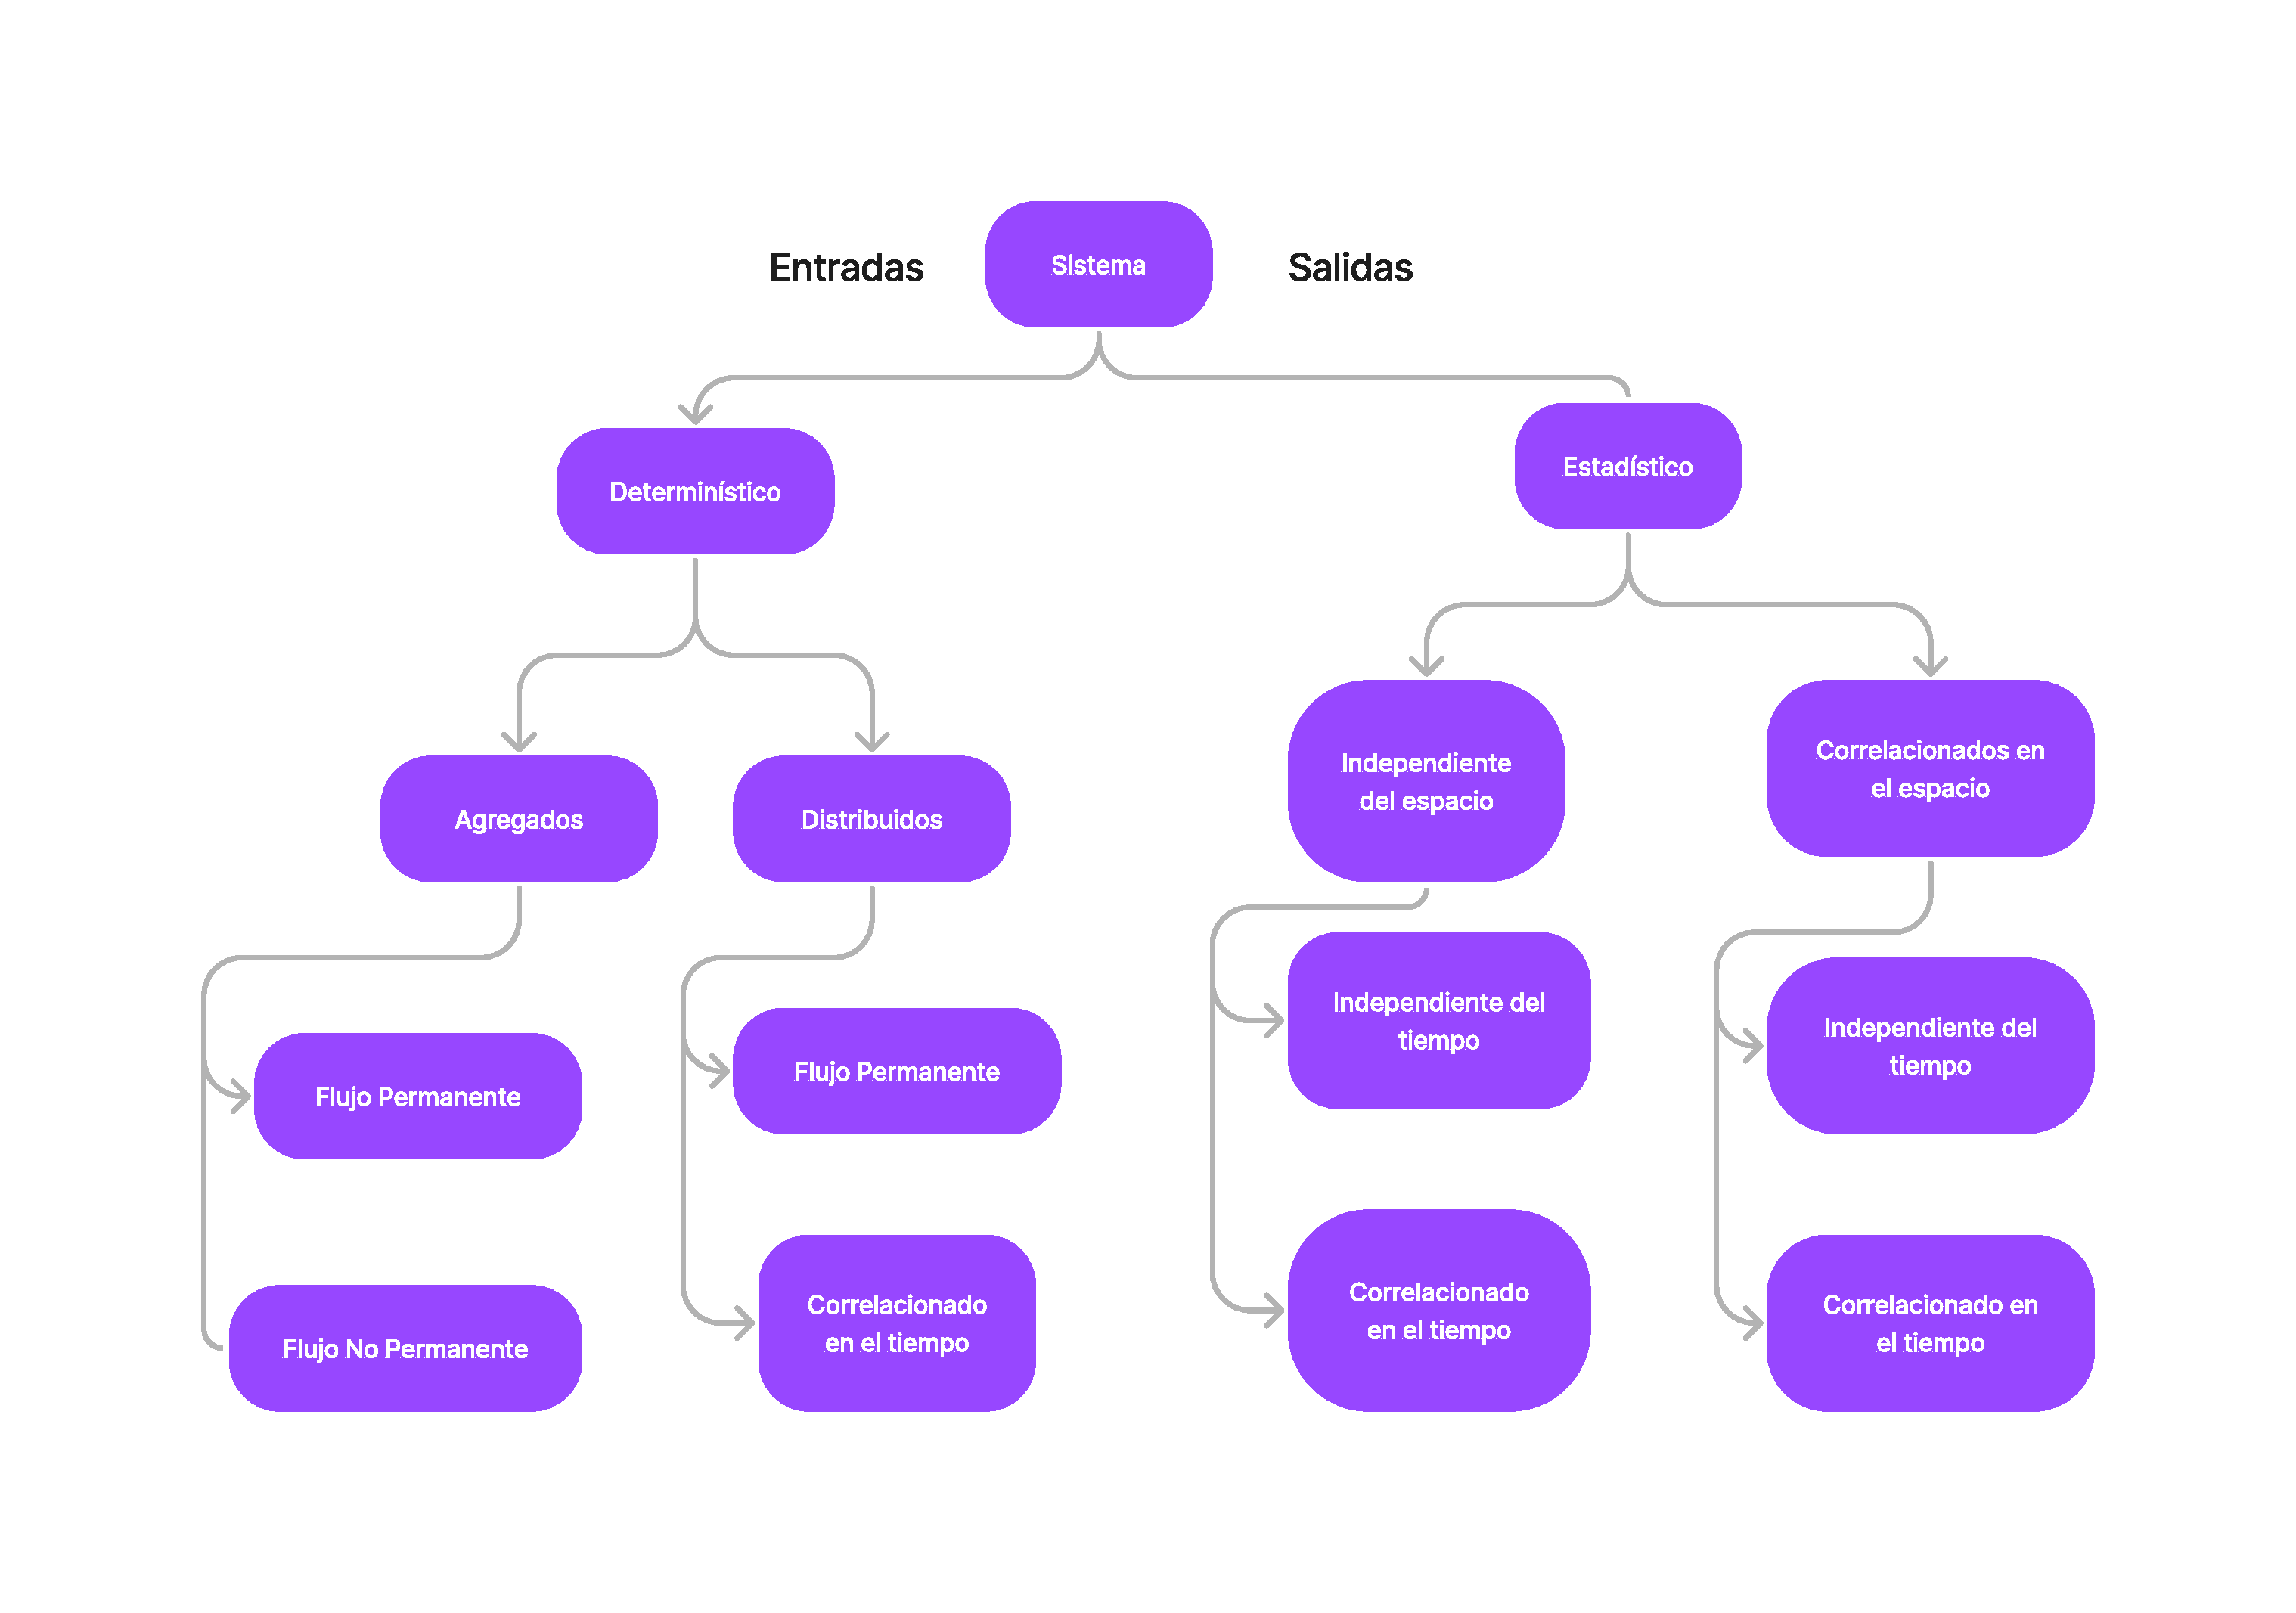
\includegraphics[width=0.8\textwidth]{csa4.pdf}
  \caption{El suelo como un sistema}
  \label{csa4}
\end{figure}
\begin{definition}[Correlación espacial]
    Una variable presenta correlación espacial cuando los valores de la variable medidos en puntos unos de otros son más parecidos que valores de la variable medidos en puntos lejanos unos de otros
\end{definition}
\begin{definition}[Correlación temporal]
    Cuando una variable presenta variación en el tiempo
\end{definition}
\subsection{Relación masa volumen primarias}
\begin{figure}[h!]
\centering
  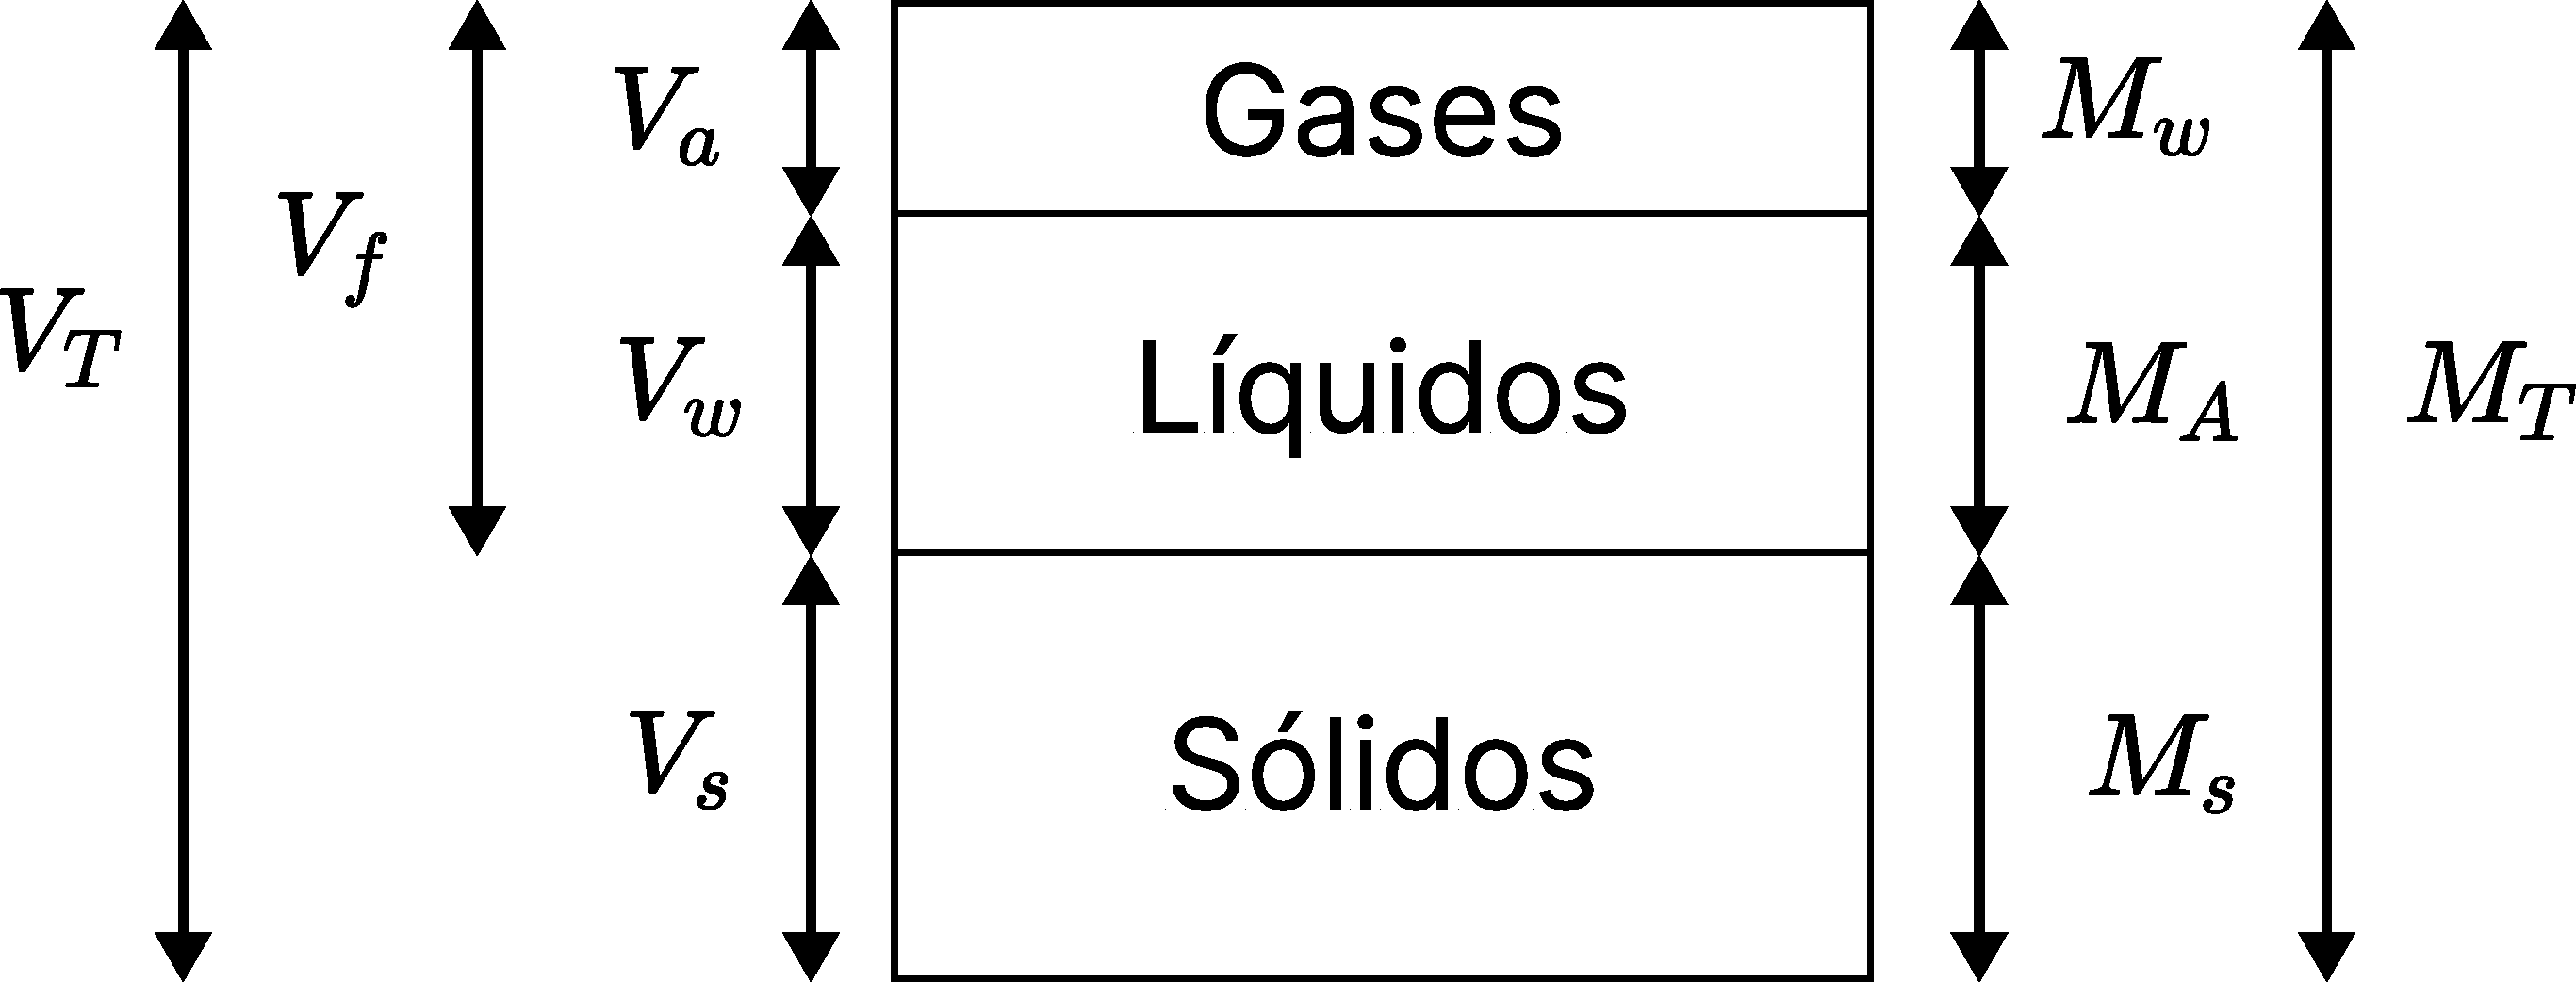
\includegraphics[width=0.5\textwidth]{csa5.pdf}
  \caption{El modelo suelo}
  \label{csa5}
\end{figure}
\begin{notation}
    \begin{itemize}
        \item $V_T$: Volumen total
        \item $V_w$: Volumen de agua
        \item $V_a$: Volumen de aire
        \item $V_s$: Volumen de sólidos
        \item $V_T$: Volumen poroso
    \end{itemize}
    Homólogamente La $m$ representa la Masa
\end{notation}
Volumen Total:
\begin{equation}
    V_T = V_w + V_a + V_s
\end{equation}
La densidad real es:
\begin{equation}
    \rho s = \frac{M_s}{Vs} = \frac{\text{Masa del suelo seco}}{\text{Volumen del suelo seco}}= \frac{g}{cm^3}
\end{equation}
$2.65gr/cm^3$ Es un valor estándar de la densidad real de un suelo ahora para la densidad aparente se calcula con la ecuación:
\begin{equation}
    \rho b = \frac{M_s}{V_T} = \frac{g}{cm^3}
\end{equation}
La ecuación de la porosidad total es:
\begin{equation}
    f = \frac{V_f}{V_T} =\frac{V_a + V_w}{V_s + V_w + V_a}= \frac{\text{Volumen poroso}}{\text{VolumenTotal}}= \frac{cm^3}{cm^3}\%
\end{equation}
La relación de vacíos, estos valores son mayores al 100\%:
\begin{equation}
    e = \frac{V_f}{V_s} = \frac{cm^3}{cm^3}\%
\end{equation}
Porosidad de aireación, cuando el sistema está saturado puede existir un valor de 0, pero el máximo $F_a$ es cuando el sistema está seco dependiendo de la porosidad puede ser 60\%.
\begin{equation}
    f_a =\frac{V_a}{V_T} = \frac{cm^3}{cm^3}\%
\end{equation}
Humedad Gravimétrica, cuando el sistema está seco puede valer 0 y alcanza su mayor valor cuando el suelo está saturado:
\begin{equation}
    \theta g = \frac{M_w}{M_{ss}} = \frac{g}{g}\%
\end{equation}
Contenido Volumétrico
\begin{equation}
    \theta v =\frac{V_w}{V_T} = \frac{cm^3}{cm^3}\%
\end{equation}
Grado de saturación
\begin{equation}
    \theta_s =\frac{V_w}{V_f} = \frac{cm^3}{cm^3}\% 
\end{equation}
\subsubsection{Relaciones masa volúmenes secundarias}
\begin{align}
    &f =\frac{\rho_s - \rho_b}{\rho_s} = 1 -\frac{\rho_b}{\rho_s}\\
    &\theta v =\frac{\theta_g \cdot \rho_b}{\rho_w}\\
    &\theta g =\frac{\theta_v \cdot \rho_w}{\rho_b}\\
    &\theta_v =\theta_s \cdot f\\
    &\rho_b =\left(1 - f\right)\rho s\\
    &e = \frac{f}{1 -f}\\
    &\theta g =\frac{M_{sh} -M_{ss}}{M_{ss}} = \frac{M_w}{M_{ss}}\\
    &f = \frac{e}{1 + e}\\
    &L = \frac{\theta_g \cdot \rho_b}{P_w}h\\
    &L =\theta_v \cdot h
\end{align}
\begin{notation}
    \begin{itemize}
        \item $f$: Porosidad Total, es el espacio de vacíos entre el volumen total
        \item $\rho_s$: Densidad Real, con valor propuesto de 2.65, masa del suelo seco entre volumen del suelo seco
        \item $\rho_b$: Densidad Aparente, masa sobre volumen, valores típicos de 1.1 a 1.7
        \item $\theta_v$: Contenido Volumétrico, volumen de agua entre volumen total
        \item $\theta_g$: Humedad Gravimétrico, masa del agua entre suelo seco
        \item $\theta_s$: Grado de saturación, Volumen de agua entre volumen poroso
        \item $f_a$: Porosidad de aireación volumen de aire entre volumen total
        \item $e$: relación de vacíos
        \item $L$: Lámina de Riego
        \item $h$: Profundidad
    \end{itemize}
\end{notation}
\subsubsection{Demostraciones}
\begin{proof}[Comprobación de $f$]
    \begin{align*}
        &f =\frac{\rho_s -\rho_b}{\rho_s} = 1 -\frac{\rho_b}{\rho_s}\\
        &f = \frac{V_f}{V_T} =\frac{V_T - V_f}{V_T} =\frac{V_T}{V_T} -\frac{V_S}{V_T} =\frac{\frac{M_S}{\rho_b}}{\frac{M_S}{\rho_b}} -\frac{\frac{M_s}{\rho_s}}{\frac{M_S}{\rho_b}} =\frac{M_S\cdot \rho_b}{M_S\cdot \rho_b} -\frac{M_S\cdot \rho_b}{M_S\cdot \rho_s} = 1 -\frac{\rho_b}{\rho_s}
    \end{align*}
\end{proof}
\begin{proof}[Comprobación de $\theta_v$]
    \begin{align*}
        &\theta_v= \frac{\theta_g\cdot \rho_b}{\rho_w}\\
        &\theta_v =\frac{V_w}{V_T} =\frac{\frac{M_w}{\rho_w}}{\frac{M_S}{\rho_b}} =\frac{M_w\cdot \rho_b}{M_s\cdot \rho_w} =\frac{M_w}{M_S}\cdot \frac{\rho_b}{\rho_w} =\theta_g\cdot \frac{\rho_b}{\rho_w} = \frac{\theta_g\cdot \rho_b}{\rho_w}
    \end{align*}
\end{proof}
% Tarea: Hacer todas las demostraciones relaciones secundarias, 12hrs  dentro de 8
\begin{proof}[$f$]
    \begin{equation}
        f = \frac{1 -\rho_b}{\rho_s}
    \end{equation}
    \begin{align*}
        &F = \frac{V_f}{V_T} = \frac{V_T - V_S}{V_T} = \frac{V_T}{V_T} - \frac{V_S}{V_T} =\frac{\frac{M_S}{\rho_b}}{\frac{M_S}{\rho_b}} -\frac{\frac{M_S}{\rho_s}}{\frac{M_S}{\rho_s}} =\\
        &\frac{M_s \cdot \rho_b}{M_s \cdot \rho_b} -\frac{M_s \cdot \rho_b}{M_s \cdot \rho_s} =\frac{1 -\rho_b}{\rho_s}
    \end{align*}
\end{proof}

\begin{proof}[$\theta_v$]
    \begin{equation}
        \theta_v = \frac{\theta_y\cdot\rho_b}{\rho_w}
    \end{equation}
    \begin{align*}
        &\theta_v = \frac{V_w}{V_T} = \frac{\frac{M_w}{\rho_w}}{\frac{M_S}{\rho_b}} = \frac{M_w}{M_S}\cdot \frac{\rho_b}{\rho_w}\\
        &\theta_g \cdot \frac{\rho_g}{\rho_w} =\frac{\rho_y\cdot\rho_g}{\rho_w}
    \end{align*}
\end{proof}

\begin{proof}[$\theta_y$]
    \begin{equation}
        \theta_y = \frac{\theta_v\cdot\rho_w}{\rho_b}
    \end{equation}
    \begin{align*}
        &\theta_y =\frac{M_w}{M_s} = \frac{V_w \cdot \rho_w}{V_T \cdot \rho_g} = \frac{V_w}{V_T} \cdot \frac{\rho_w}{\rho_g} =\theta_v \cdot \frac{\rho_w}{\rho_g}\\
        &=\frac{\theta_v \cdot \rho_w}{\rho_g}
    \end{align*}
\end{proof}

\begin{proof}[$\theta_v$]
    \begin{equation}
        \theta_v =\theta_s \cdot f
    \end{equation}
    \begin{align*}
        &\theta_v = \frac{V_w}{\frac{V_f}{f}} = \frac{V_w \cdot f}{V_f} =\\
        &\frac{V_w}{V_f} \cdot f = \theta_s \cdot f
    \end{align*}
\end{proof}

\begin{proof}[$\theta_v$]
    \begin{equation}
        \theta_v = f - F_a
    \end{equation}
    \begin{align*}
        &\theta_v = \frac{V_w}{V_T} = \frac{V_w + V_a - V_a}{V_T} = \frac{V_w - V_a}{V_T} - \frac{V_a}{V_T}\\
        &\frac{V_f}{V_T} - \frac{V_a}{V_T} = f - F_a
    \end{align*}
\end{proof}

\begin{proof}[$\rho_b$]
    \begin{equation}
        \rho_b = \left(1 - f\right) \cdot \rho_s
    \end{equation}
    \begin{align*}
        pendiente
    \end{align*}
\end{proof}

\begin{proof}[$e$]
    \begin{equation}
        e = \frac{f}{1 - f}
    \end{equation}
    \begin{align*}
        &e = \frac{V_f}{V_s} = \frac{V_f}{V_T - V_F}\\
        &\frac{\frac{V_f}{V_T}}{\frac{V_T}{V_T} - \frac{V_f}{V_T}} = \frac{f}{1 - F}
    \end{align*}
\end{proof}

\begin{proof}[$\theta_g$]
    \begin{equation}
        \theta_g = \frac{M_{sh} - M_{ss}}{M_{ss}}
    \end{equation}
    \begin{align*}
            &\theta_g =\frac{M_w}{M_{ss}}\\
            &=\frac{M_w - M_{ss} + M_{ss}}{M_{ss}}\footnote{Considerando que $M_{sh} = M_w + M_{ss}$} =  \frac{M_{sh} - M_{ss}}{M_{ss}}
    \end{align*}
\end{proof}

\begin{proof}[$f$]
    \begin{align*}
        &f = \frac{e}{1+ e}\\
        &F = \frac{V_f}{V_T} = \frac{V_f}{V_f + V_s} = \frac{\frac{V_f}{V_s}}{\frac{V_f}{V_s} + \frac{V_s}{V_s}} = \frac{e}{ 1 + e}
    \end{align*}
\end{proof}


\begin{proof}[$\rho_b$]
    \begin{equation}
        \rho_b =\left(1- f\right) \cdot \rho_s
    \end{equation}
    \begin{align*}
        &\rho_b =(1 - f)\rho_s =\frac{M_s}{V_T}\\
        &\left(1 - \frac{V_f}{V_T}\right)\cdot \frac{M_s}{V_s}\\ 
        &\frac{M_s}{V_s} -\frac{M_s \cdot V_f}{V_T\cdot V_s}\\
        &\frac{M_s \cdot V_T \cdot V_S - M_s \cdot V_F \cdot V_S}{V_T \cdot V_S^2} =\\
        &\frac{V_S\left(M_S \cdot V_T - M_S \cdot V_F\right)}{V_T \cdot V_s^2} =\frac{M_S\left(V_T - V_F\right)}{V_T \cdot V_S}\\
        &\frac{M_S}{V_T}\cdot \frac{V_T - V_F}{V_S} = \frac{M_S}{V_T} \cdot \frac{V_S + V_w + V_a - V_a - V_w}{V_S} =\\
        &\frac{M_S}{V_T} =\rho_b 
    \end{align*}
\end{proof}







\subsubsection{Densidad aparente y densidad real}
Su valor se utiliza para el cálculo de la porosidad total del suelo, inferir procesos de compactación del suelo, calcular la masa de un suelo en un área con una profundidad determinada y el cálculo del carbono capturado por un suelo
\subsubsection{Cálculo de la macroporosidad y la microporosidad del suelo}
¿Cuál es la porosidad de un suelo sí?
\begin{align*}
    &\rho_b = \frac{1.1gr}{cm^3}\\ 
    &\rho_s = \frac{2.65gr}{cm^3}\\
    &f = 1 -\frac{\rho_b}{\rho_s} = 1 -\frac{1.1}{2.65} = 0.5849\\
    &f = 58.49\%
\end{align*}
\begin{example}
    ¿Cuál es la macroporosidad y la microporosidad de un suelo con las siguientes características?
    \begin{itemize}
        \item $f=58.49\%$
        \item $CC=29\%$
        \item $f=M+m$
    \end{itemize}
\end{example}
\textit{ Sol. }
\begin{align*}
    &m =\frac{CC \cdot \rho_b}{\rho_w} = \frac{0.29 \cdot 1.1}{1} = 0.319\\
    &m = 31.90\implies M = f- m = 58.49 - 31.90 = 26.59\%
\end{align*}
\begin{definition}[Capacidad de Campo]
    Punto técnico de movimiento y no movimiento del suelo, es un valor de $\theta_g$ contenido gravimétrico en el sistema
\end{definition}
\subsubsection{Calcular la masa de un suelo en un área y con una profundidad determinada}
\begin{example}
    
¿Determine la cantidad suelo erosionada, si en un terreno se perdió una lámina de 0.5cm, el terreno tiene un área de 10Ha?
\end{example}
\textit{ Sol. }
\begin{align*}
    &\rho_b =\frac{1.2g}{cm^3}\\
    &\rho_b = \frac{M_S}{V_T}\\
    &M_S =\rho_b\cdot V_T\\
    &V_T = A\cdot h =\left(100,000m^2\right)\left(0.005m\right) = 500m^3\\
    &M_S =\left(\frac{1.2ton}{m^3}\right)\left(500m^3\right) = 600ton\\
    &\frac{1,000,000g}{1,000,000cm^3} = \frac{1ton}{1m^3}
\end{align*}
\subsubsection{Calcular la cantidad de carbono capturado por un suelo en un área y profundidad}
\begin{example}
    Se tiene un suelo donde:
    \begin{enumerate}
        \item \% de Materia Orgánica es de 5\%
        \item Profundidad de 50cm
        \item Densidad aparente de $\frac{1.3gr}{cm^3}$
        \item Área de 1 Ha
    \end{enumerate}
\end{example}

\textit{ Sol. }
Se calcula la masa de los sólidos
\begin{align*}
    &\rho_b = \frac{M_s}{V_T}\\
    &M_S = \rho_b\cdot V_T\\
    &V_T = A\cdot h =\left(100,000m^2\right)\left(0.50m\right) = 5000m^3\\
    &M_S =\left(\frac{1.3ton}{m^3}\right)\left(5000m^3\right) = 6,500ton\\
\end{align*}
Posteriormente se debe calcular la cantidad de carbono orgánico con base en el dato de \% Materia Orgánica:
\begin{equation*}
    \%C_{org} =0.58\left(\%\text{de M.O.}\right)=0.58\left(5\%\right)2.9\%
\end{equation*}
Finalmente se obtiene la cantidad de carbono capturado por el suelo considerando una Ha, aplicando:
\begin{equation*}
C_{\text{org capturado}}=M_S\left(\%\text{ de C capturado}\right)=6,500t(0.029) = \frac{188.5ton}{Ha}
\end{equation*}
Otra forma más directa es aplicando:
\begin{align*}
    C_{\text{org capturado}}=\left(0.029\right)\left(\frac{1.3ton}{m^3}\right)\left(10,000m^2\right)\left(0.5m\right) = 188.5ton/Ha
\end{align*}
Y otra manera más es aplicando:
\begin{equation*}
    C_{\text{org capturado}}=\left(\% \text{de C org}\right)\left(\rho_b\right)\left(Profundidad\right) = 2.9 \cdot 1.3 \cdot 50 =188.5ton/Ha
\end{equation*}

\begin{problem}[Relación Masa Volumen del suelo]
    Una muestra de suelo húmeda teniendo una masa de 1,000gr y un volumen de $640cm^3$ fue secada, teniéndose una masa de suelo seco de 800g. Asumiendo un valor de $2.65g/cm^3$ de densidad real y una densidad del agua de $1.0g/cm^3$ obtenga $\rho_b,f,e,\theta_g\theta_v\theta_s,f_a$
\end{problem}

\textit{ Sol. }
Se trata de un Suelo franco
\begin{align*}
    &\rho_b = \frac{M_s}{V_T} =\frac{800gr}{640cm^3} = 1.25\\
    &f =1 - \frac{\rho_b}{\rho_s} = 1 -\frac{1.25}{2.65} = 0.5283=52.83\%\\
    &e = \frac{V_f}{V_s} =\frac{f}{1 - f} =\frac{0.5283}{1 -0.5283} = 1.11 = 112\%\\
    &\theta_g = \frac{M_w}{M_{ss}} = \frac{200}{800} = 0.25 = 25\%\\
    &\theta_v = \frac{V_w}{V_T} = \frac{200cm^3}{640cm^3} =0.3125 = 31.25\%\\
    &\theta_s = \frac{V_w}{V_f = f\cdot V_T} = \frac{200cm^3}{338.112cm^3} = 0.5915 = 59.15\%\\
    &f_a = \frac{V_a}{V_T} = \frac{138.12}{640cm^3} = 0.2158 = 21.58\%
\end{align*}
%¿Por qué siempre el contenido volumétrico es mayor que el gravimétrico?
%Es necesario tener clara las relaciones primarias con $\theta_g$
%¿Qué significa un grado de saturación del 50\%?
\begin{example}
    Cuántos centímetros de agua están contenidos en un perfil de un suelo o un metro de profundidad, si el contenido de humedad gravimétrico en los 40cm seuperiores es del 15\% y en los 60cm inferiores es de 25\%. La densidad aparente en la capa superior es de $1.2 g/cm^3$ y en la inferior es de $1.4g/cm^3$. ¿Cuánta agua contiene el sielo por Ha dada como en volumen en litros?
\end{example}
\begin{figure}[h!]
\centering
  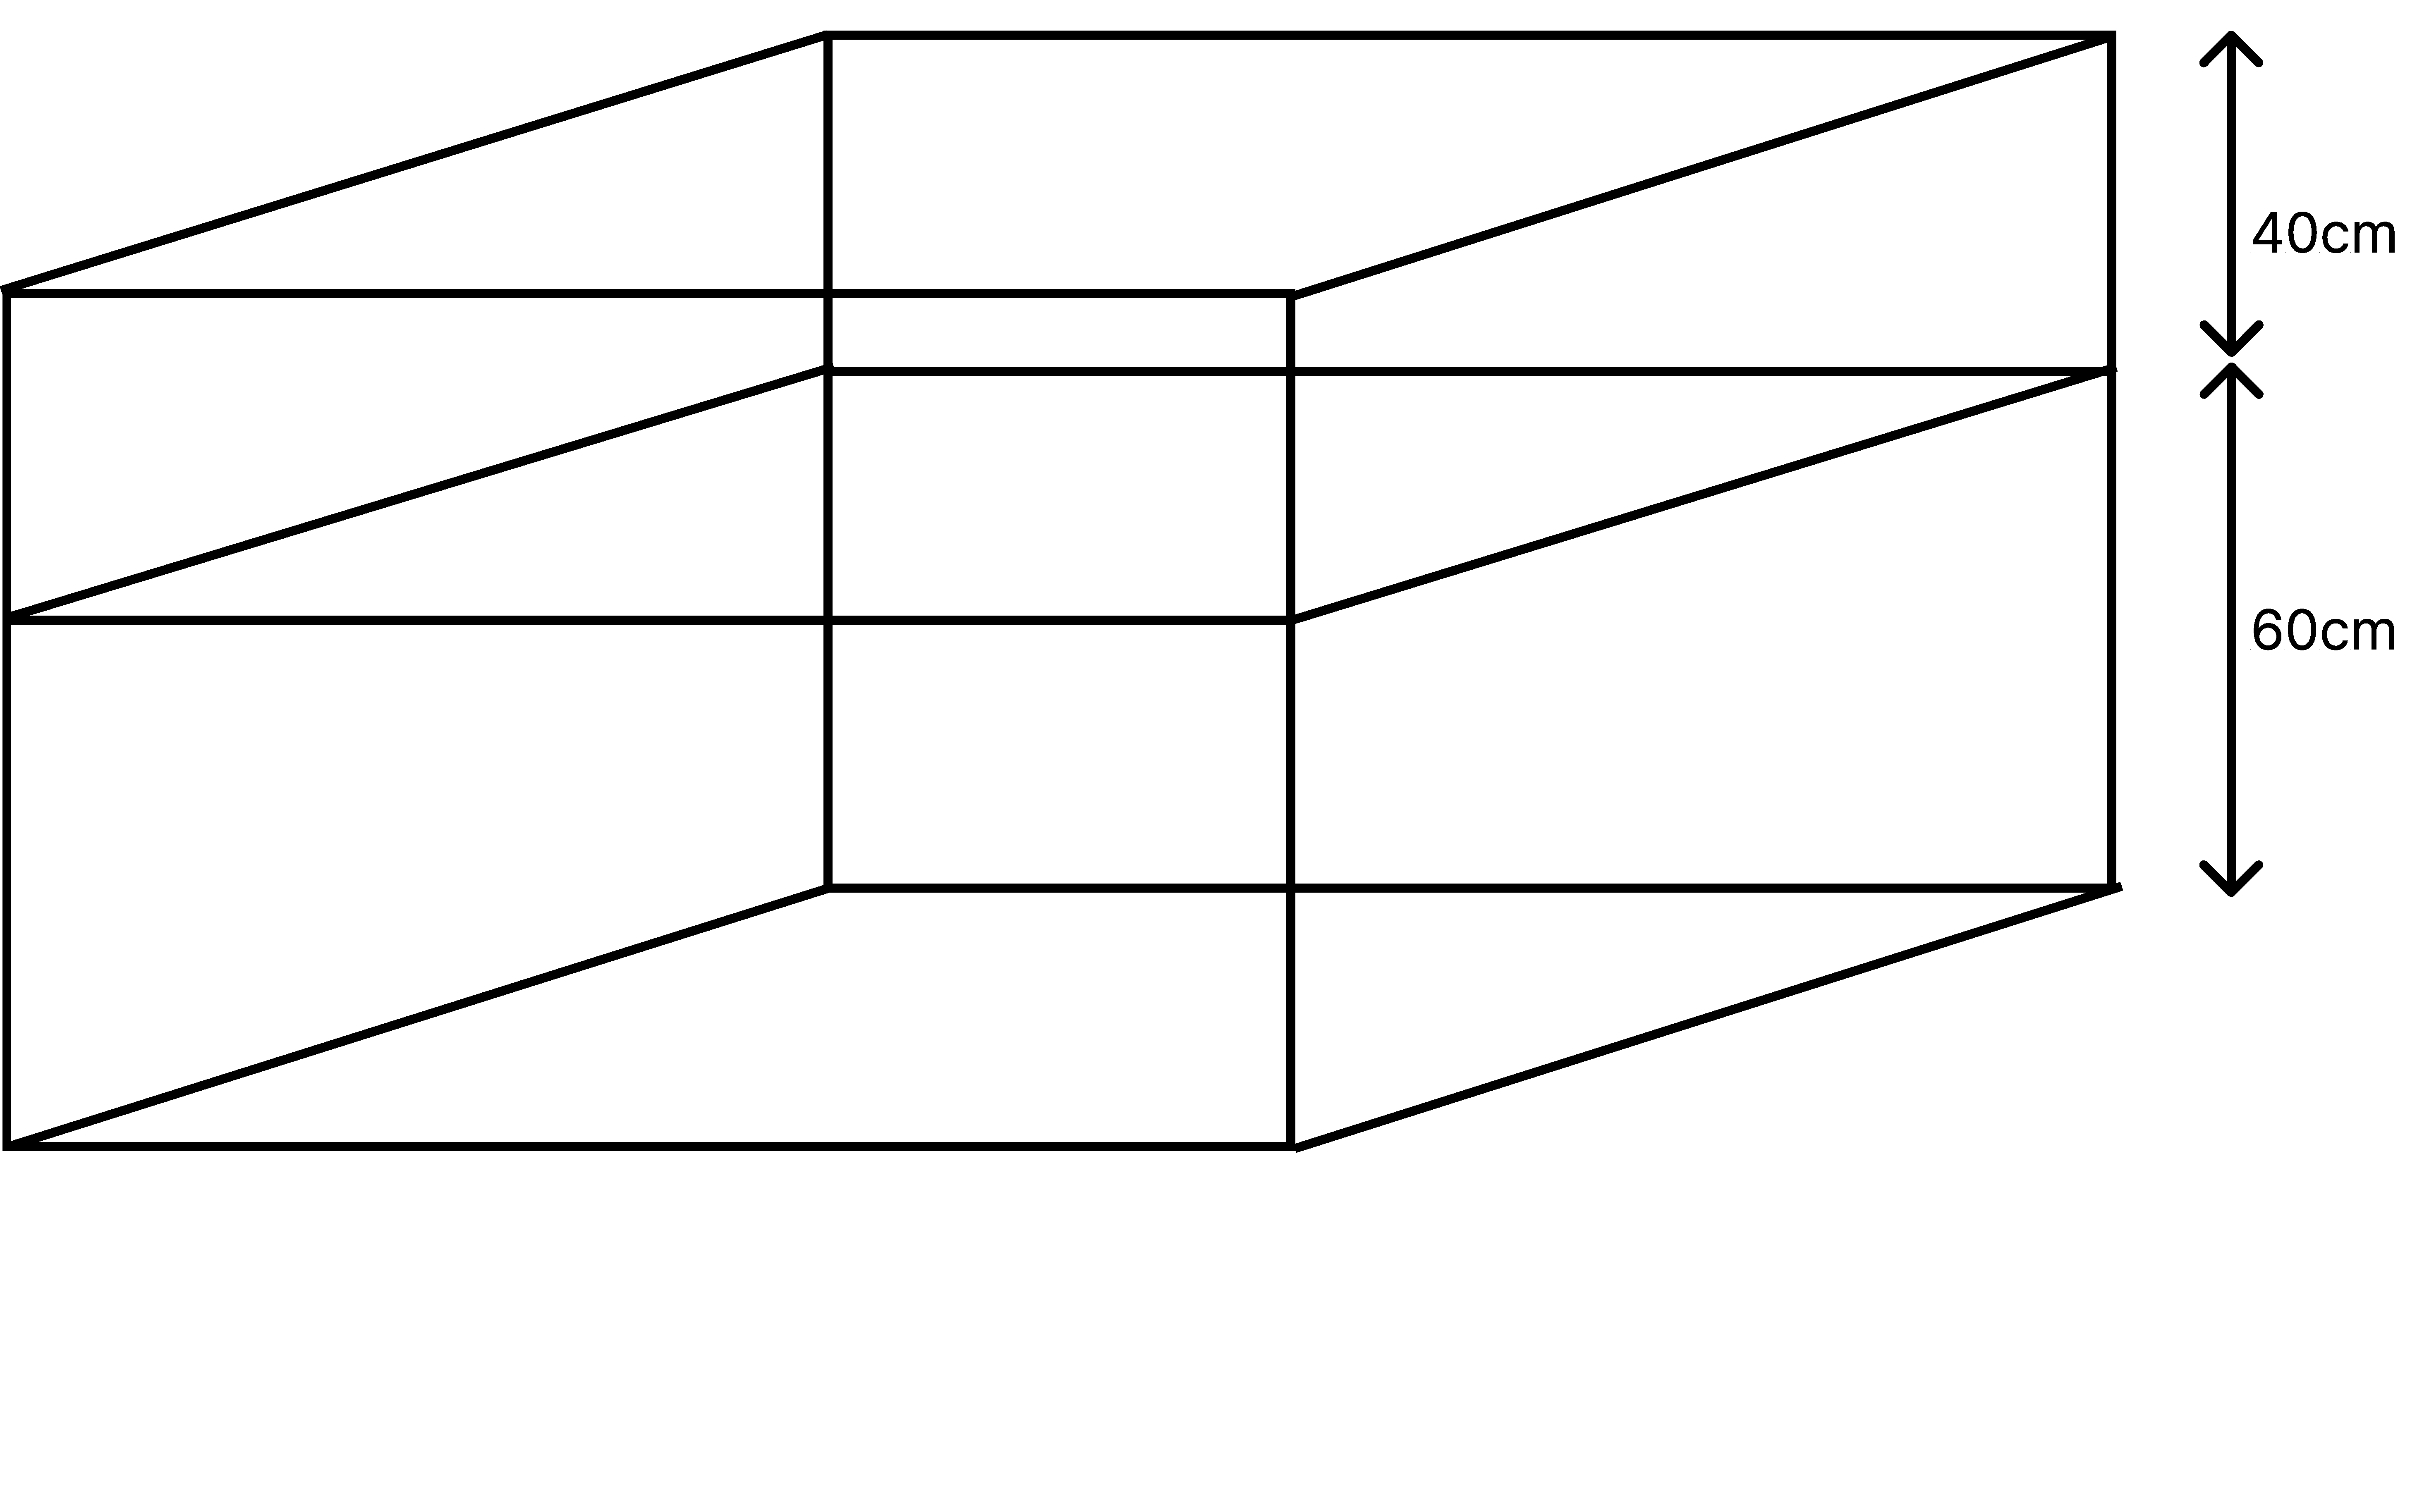
\includegraphics[width=0.5\textwidth]{csa6.pdf}
  \caption{Esquema del problema}
  \label{cas6}
\end{figure}
\textit{ Sol. }

Para resolver el problema se utiliza la fórmula de lámina que afirma:
\begin{equation*}
    L= \frac{\theta_g\cdot \rho_b}{P_w}\cdot h
\end{equation*}
Para los 40cm superiores:
\begin{equation*}
    L =\frac{0.15 \cdot 0.12}{1.0} \cdot 40 = 4.2cm
\end{equation*}
Para los 60cm inferiores:
\begin{equation*}
    L = \frac{0.25 \cdot 1.4}{1.0} \cdot 60 = 21cm
\end{equation*}
Por lo tanto, $7.2 + 1.0 = 28.2cm$, el agua que contiene el sistema por ha dad en $m^3$ y en litros es:
\begin{equation*}
    V =A \cdot L_{Total} = 10,000m^3 \cdot 0.282m = 2,820,000L
\end{equation*}

\subsection{Composición mecánica}

El componente mineral clasificado por:
\begin{itemize}
    \item Tamaño
    \item Forma
    \item Composición química
\end{itemize}

\subsubsection{Tamaño}
Las partículas individuales que forman, puede ser clasificadas por su tamaño en:
\begin{itemize}
    \item Rocas o piedras: partículas mayores a 2cm
    \item Gravas: partículas entre 2cm-2mm
    \item Suelo fino: partículas menores de 2mm
\end{itemize}
A su vez, el suelo fino se subdivide en arenas, limos y arcillas
\begin{table}[h!]
    \centering
    \begin{tabular}{@{}cc@{}}
    \toprule
    Textura                                          & Rango                                      \\ \midrule
    \multicolumn{2}{c}{\textbf{\begin{tabular}[c]{@{}c@{}}USDA\\ (Diámetros en mm)\end{tabular}}} \\
    Arena muy gruesa                                 & 2.00-1.00                                  \\
    Arena gruesa                                     & 1.00-0.50                                  \\
    Arena media                                      & 0.50-0.25                                  \\
    Arena fina                                       & 0.25-0.10                                  \\
    Arena muy fina                                   & 0.10-0.05                                  \\
    Limos                                            & 0.05-0.002                                 \\
    Arcillas                                         & >-0.002                                    \\
    \multicolumn{2}{c}{\textbf{\begin{tabular}[c]{@{}c@{}}ISSS\\ (Diámetros en mm)\end{tabular}}} \\
    Arena gruesa                                     & 2.00-0.20                                  \\
    Arena fina                                       & 0.20-0.02                                  \\
    Limos                                            & 0.02-0.002                                 \\
    Arcillas                                         & <-0.002                                    \\ \bottomrule
    \end{tabular}
    \caption{Composición mecánica}
    \label{tabcsa5}
\end{table}
\subsection{Granulometría}
La granulometría de suelos se refiere a la distribución por tamaño y porcentaje de las partículas que componen un suelo. Según la composición del suelo,la granulometría puede determinarse por dos métodos fundamentales:
\begin{itemize}
    \item Vía seca: Partículas por arriba de 0.074mm (Se utilizan tamices)
    \item Vía húmeda: Partículas por abajo de 0.074 mm (Se utiliza la sedimentación fraccionada: Ley de Stokes)
\end{itemize}
\begin{enumerate}
    \item Tomar una muestra representativa del sistema de 500gr
    \item Secar la muestra al aire
    \item Tomar 300 gramos del material y colocarlos en el tamiz superior del tren de tamizado, con los tamices ordenados iniciando de la parte superior de mayor a menor abertura, el último tamiz deberá ser de 0.074mm y en la parte inferior de la charola
    \item Poner a funcionar el tren por 10 minutos
    \item Detener el tamizado y cuantificar la cantidad de material retenido en cada tamiz
\end{enumerate}
\begin{figure}[h!]
\centering
  \includegraphics[width=0.5\textwidth]{csa7.jpg}
  \caption{Curva granulométrica}
  \label{csa7}
\end{figure}
La curva granulométrica de un suelo es una representación gráfica de los resultados obtenidos en un laboratorio cuando se analiza la estructura del suelo desde el punto de vista del tamaño de las partículas que lo forman, véase la figura \ref{csa7}.

Existen diferentes métodos de análisis textural pero los que más se utilizan en México son:
\begin{enumerate}
    \item pipeta
    \item Hidrómetro de Bouyoucos
    \item Hidrómetro modificado por Day
\end{enumerate}
Están basados en el proceso de sedimentación fraccionada de partículas que tiene com base matemática la Ley de Stokes

Cuando una partícula sólida de forma esférica cae dentro de un fluido se ejercen las siguientes fuerzas:
\begin{itemize}
    \item Peso de la partícula $(P)\downarrow$
    \item Empuje del líquido $(E)\uparrow$
    \item Fierza resistente al movimiento $(R)\uparrow$
\end{itemize}
Entonces:
\begin{equation}
    P=\frac{4}{3}\pi\cdot r^3\cdot\rho_s\cdot g
\end{equation}
\begin{equation}
    E=\frac{4}{3}\pi\cdot r^3\cdot \rho_l\cdot g
\end{equation}
\begin{equation}
    R=6\cdot \pi\cdot\nu\cdot r\cdot v
\end{equation}
\begin{notation}
\begin{itemize}
    \item $R=$ Radio (cm)
    \item $\rho_s=$ Densidad del sólido $(g/cm^3)$
    \item $g=$ Constante gravitacional $(g/cm^3)$
    \item $\rho_l=$ Densidad del líquido $(g/cm^3)$
    \item $\nu=$ Viscosidad (Poises) $g/(cm\cdot s)$
    \item $V$= Velocidad (cm/s)
\end{itemize}
\end{notation}
\begin{proof}[Ley de Stokes]
    \begin{equation}
        V = \frac{2r^2\cdot g\left(\rho_s - \rho_l \right)}{9\nu} = \frac{d^2\cdot g\left(\rho_s -\rho_l\right)}{18\nu}
    \end{equation}
    % TODO: PENDIENTE
\end{proof}
\subsection{Textura con separación de arenas}
\begin{enumerate}
    \item Tomar la cantidad adecuada de suelo
    \item Realizar la dispersión química
    \item Realizar la dispersión física
    \item Aplicar el método elegido
\end{enumerate}
De una muestra de 100 gr, se separa la materia orgánica y a lo resultante, se tomará 40gr. Se tomará cerca de 11 lecturas

\begin{definition}[Hidrómetro]
    Es un densímetro calibrado para medir grados de materiales en suspensión al centro del Bulbo
\end{definition}

\subsubsection{Método del hidrómetro de Bouyoucos}
El método consiste en la utilización de un hidrómetro que n es más que un densímetro que consta de un bulbo y un vástago graduado con unidades desde 60 a -5
\begin{enumerate}
    \item Utilizar 50 gr de suelo
    \item A los 40 segundos de iniciado el proceso de sedimentación se lee \% (L+R)
    \item A las 3 horas de iniciado el proceso de sedimentación se lee \% (R)
\end{enumerate}
El hidrómetro está calibrado para leer gramos de suelos en suspensión, para 100g de suelo y una temperatura específica, generalmente $20^{\circ}C$ con las lecturas de los porcentajes de L+R y R, entonces
\begin{itemize}
    \item Primera lectura*2=\%(LR)
    \item Segunda lectura*2=\%R
    \item $\% L= \%\cdot (L+R)-\% R$
    \item $\% A= 100-\%\cdot (L+R)$
\end{itemize}
Este método es sencillo y su validez está dada por la relación que existe entre la concentración de una suspensión de suelo y su densidad
Por ejemplo, en el triángulo de textura, determinamos que R=13\%, L=30\%-13\%=17\% y por lo tanto A=100\%-30\%=70\%
Para separar arenas se toma un tren de tamices, con los diámetros límites de cada una de las clases de arena

\subsection{Estructura y dispersión}

\subsubsection{Estructura de las arcillas}

\begin{definition}[Unidad tetraédrica]
    Constituida por cuatro átomos de oxígeno equidistantes de un átomo de Silicio. Estas unidades se pueden combinar para formar una lámina conocida como sílica se representa mediante un trapecio
\end{definition}
\begin{figure}[h!]
\centering
  \includegraphics[width=0.5\textwidth]{csa8.png}
  \caption{Unidad tetraédrica}
  \label{csa8}
\end{figure}
\begin{definition}[Unidad Octaédrica]
    Constituida por seis Hidróxilos (OH) rodeando a un átomo que puede ser aluminio (Al) o magensio (Mg). Esta unidad se puede combinar con otras para formar láminas de octaédricas, en los que si el catión central es Mg se denomina brucita, si es Al se denomina Gibsita, las láminas se representan mediante un rectángulo
\end{definition}
\begin{figure}[h!]
\centering
  \includegraphics[width=0.3\textwidth]{csa9.png}
  \caption{Unidad Octaédrica}
  \label{csa9}
\end{figure}
\begin{enumerate}
    \item Una lámina octaédrica con una tetraédrica es denominada arcilla 1:1, por ejemplo la Caolinita no expandible.
    \item Dos laminas octaédrica con una tetraédrica es una arcilla 2:1, por ejemplo la Montmorillonita y las Illitas, este último fija potasio y tiene menor expansión
\end{enumerate}
\subsubsection{Arcillas Caolinitas (1:1)}

\begin{figure}[h!]
\centering
  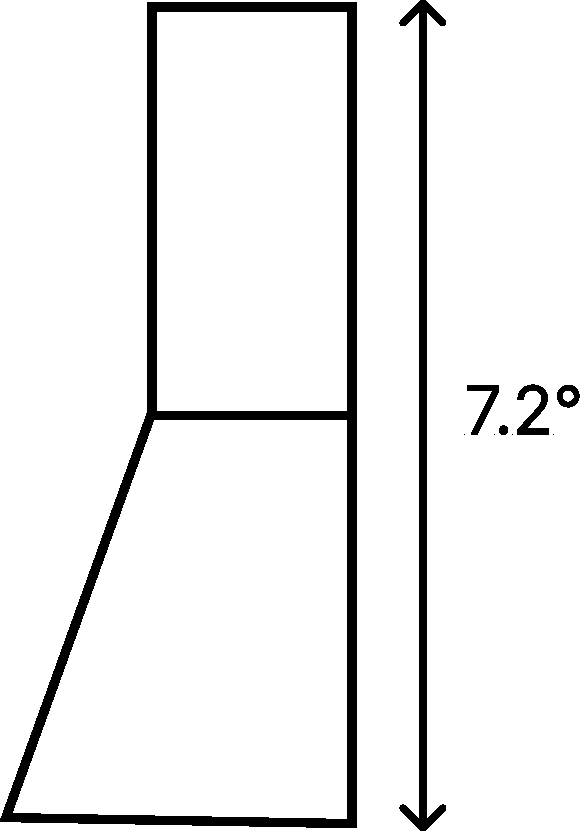
\includegraphics[width=0.2\textwidth]{csa10.pdf}
  \caption{Arcillas Caolinitas (1:1), el rectangulo representa un octaedro y el trapecio un tetraedro}
  \label{csa10}
\end{figure}
La lámina silicea se une a una de gibsita, el mineral que se obtiene es llamado caolin; cuando se unen caolines uno sobre otra forman la caolinita. Las fuerzas que unan las láminas de caolin para formar la caolinita son del tipo puente de hidrógeno que se forma entre los iones de $O^{-2}$ y $OH^-$ esta unión es relativamente fuerte; las fuerzas que unen la gibsita y silica son del tupo valencia, las cuales son 10 veces más fuertes que los del tipo puente de hidrógeno. En este tipo de arcilla las carga neta negativa son los bordes de rompimiento y la disociación del OH en presencia de agua liberando el H.
\subsubsection{Arcillas Motmorillonitas (2:1)}
\begin{figure}[h!]
\centering
  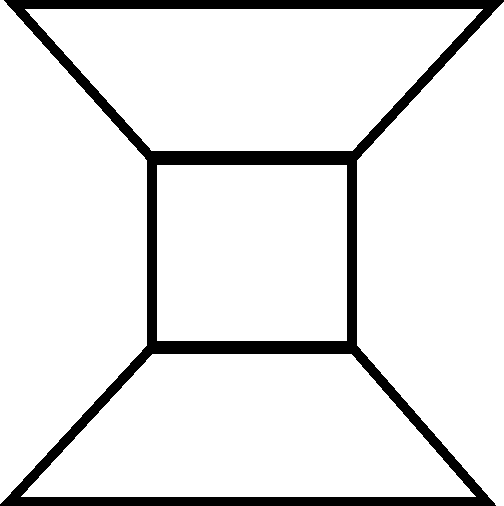
\includegraphics[width=0.2\textwidth]{csa11.pdf}
  \caption{Arcillas Motmorillonitas (2:1)}
  \label{csa11}
\end{figure}
En estas arcillas se unen dos láminas de silica (tetraédricos) a una de gibsita (octaédrica) el mineral obtenido se conoce como pirofilita, las pirofilitas s eunen unas a otras teniendo como elementos de liga a los cationes intercambiables, esta unión por lo general es débil, por lo que el agua puede entrar fácilmente entre las láminas por lo que se presenta el fenómeno de expansión.

En este tipo de arcilla la pirofilita es neutra, pero el origne de las cargas negativas es la sustitución isomórdica que ocurre en la capa octaédrica, y consiste en la entrada de $Fe^{2+}$ y $Mg^{+2}$ y la salida de $Al^{3+}$
\subsubsection{Acrillas Illíticas (2:1)}
La unidad estructural es semejante a la motmorillonita, pero se presenta una sustitución usomorda adicional en la lámina tetraédrica, de átomos de $Si^{+4}$, resultando una carga negativa más alta que en la motmorillonita; sin embarho una parte sustancial de esta carga se equilibra con átomos de $k^{+}$ no intercambiable que le dan una liga fuerte entre las láminas de pirofilita, debido a esto la ilita no se expande y se dice que fija el $k+$
\subsection{Propiedades electrocinéticas de la Arcilla}
\subsubsection{Doble capa eléctrica y potencial Z}

Las partículas de arcilla poseen una vcarga negatica neta debido a:
\begin{enumerate}
    \item BOrdes de rompimiento
    \item Ionización de los OH
    \item Sustitución isomórfica
\end{enumerate}
Las cargas negativas sobre la superficie de las arcillas y los cationes intercamibables forman una doble capa eléctrica alrededor de las partículas.

H.Von Helmholtz sugirió en 1874 que la doble capa eléctrica tenía un grosor fijo (rígido)
\begin{figure}[h!]
    \centering
      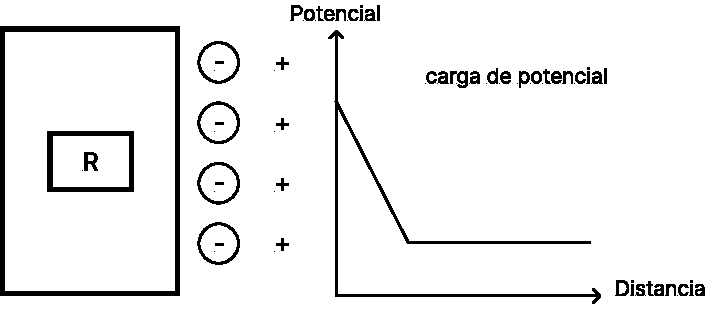
\includegraphics[width=0.5\textwidth]{csa12.pdf}
      \caption{Estructura lineal}
      \label{csa12}
    \end{figure}
    El modelo fue inadecuado y G Gouy y D.L. Chapman propusieron una capa doble difusa donde la concentración de iones + cerca de la superficie era alta y a medida que se aleja de la superficie la concentración decrece hasta que la densidad de carga neta es cero
    \begin{figure}[h!]
    \centering
      \includegraphics[width=0.5\textwidth]{csa13.pdf}
      \caption{Estructura curva}
      \label{csa13}
    \end{figure}
    O. Sern (1924) mostró que ninguna de las teorías por sí sola era adecuada y propuso la combinación de ambas teorías.
    \begin{figure}[h!]
    \centering
      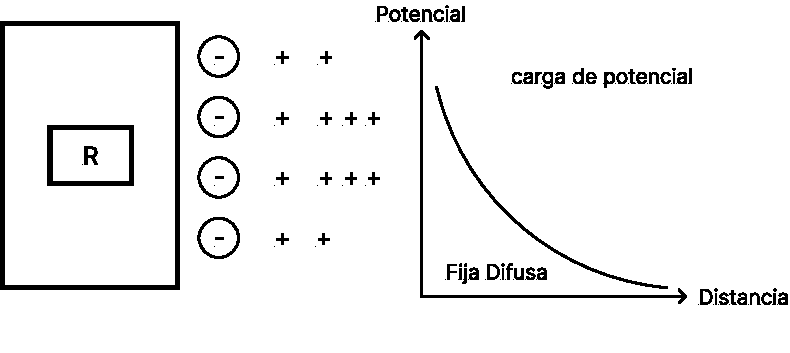
\includegraphics[width=0.5\textwidth]{csa14.pdf}
      \caption{Teoría de la doble capa eléctrica}
      \label{csa14}
    \end{figure}
    El grosor impide que las capas floculen, a partir de que se da esa unión es que se forman las estructuras.
    Los cationes monovalentes engrosan las capas eléctricas, los bivalentes y trivalentes como calcio y magnesio son excelentes para disminuir esa capa eléctrica, u otra.
    \begin{definition}[Estructura]
        Es una propiedad que lo caracteriza al igual que el color o la textura, la diferencia, es que la estructura es una propiedad dinámica que puede cambiar en respuesta a las condiciones del medio natural y las prácticas de manejo del suelo.
    \end{definition}
    El rango de tamaño de partículas estudiadas es muy amplio, desde las partículas arcillosas con dimensiones de $10^{-7}$m hasta terrones de 2cm, por lo tanto se concluye que la estructura del suelo es la unión de partículas primarias, en partículas compuestas llamadas agregados, los cuales están separados unos de otros por superficies de ruptura.
    \begin{definition}[Agregado]
        Es un grupo de partículas individuales, las cuales son retenidas juntas por fuerzas de diferente naturaleza, pero que en conjunto son mayores que las fuerzas entre los agregados adyacentes, un agregado individual se denomina ``Ped''
    \end{definition}
    El estudio de la estructura del suelo trata con la organización de las partículas primarias en agregados y con la estabilidad de estos agregados, ante agentes que pudieran destruirlos y por tanto deteriorar la estructura.
    
    \begin{figure}[h!]
    \centering
      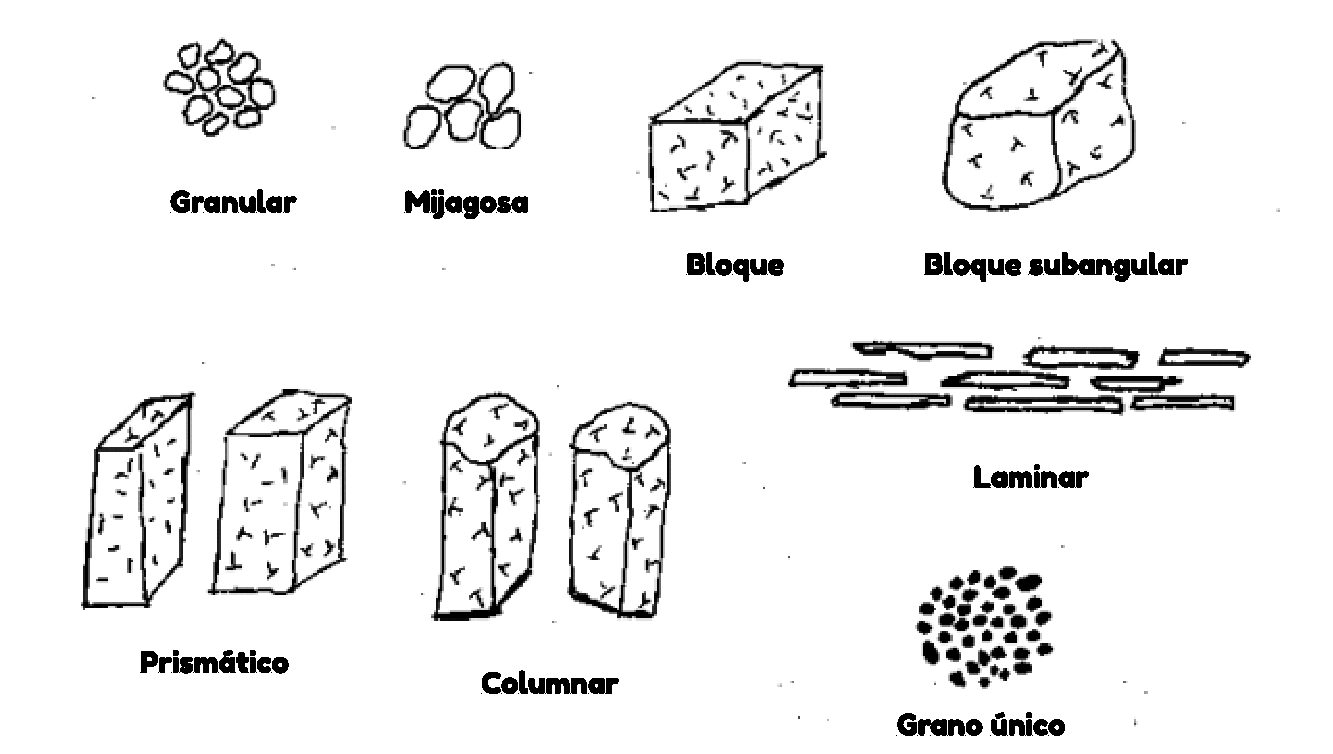
\includegraphics[width=0.5\textwidth]{csa15.pdf}
      \caption{Tipos de estructura}
      \label{csa15}
    \end{figure}
    El tamaño de los agregados varía desde un diámetro de micras hasta varios cm, pero podemos identificar tres niveles de agrupamiento de acuerdo a su tamaño
    \begin{itemize}
        \item Nivel de dominios: Unión de arcillas
        \item Nivel de microagregados: Unión de arcillas con limos y arenas
        \item Nivel de macroagregados: Unión de microagregados
    \end{itemize}
    En el primer nivel de participación, sólo arcillas, las cuales se suponen que forman los dominios;
    
    El segundo nivel se subdivide en: \begin{itemize}
        \item Microestructura fina: Agregados de menos de 0.01mm de diámetroMicroestructura gruesa: Agregados de 0.01mm-0.25mm de diámetro
    \end{itemize}
    En el último nivel se subdivide en \begin{itemize}
        \item Macroestructura: Agregados de 0.25mm a 10mm de diámetro
        \item Megaestructura: Agregados de más de 10mm de diámetro
    \end{itemize}
    En el suelo hay fuerzas que intervienen para unir los agregados:
    \begin{itemize}
        \item Magnéticas
        \item Electroestáticas
        \item Moleculares o de Vander Waals
        \item Capilares
        \item Iono-electrostáticas
        \item Químicas (Valentes)
    \end{itemize}
    Los mecanismos de formación de la estructura en los suelos son diferentes por lo que no sería correcto hablar de la génesis de la estructura como una teoría única aunque hace algunos años se establecieron tres teorías que son las siguientes:
    \begin{enumerate}
        \item Agregación por coagulación
        \item Cementación
        \item Capilaridad
    \end{enumerate}
    Ninguna de estas tres teorías por sí sola la agregación del suelo y la formación de la estructura entonces más que habla de una teoría única de la génesis de la estructura se tendría que hablar sobre los agentes de agregación, que son las siguientes:
    \begin{itemize}
        \item Floculación
        \item Arcillas
        \item Cementantes inorgánicos
        \item Iones intercambiables (Cationes)
        \item Cementantes orgánicos
        \item Microorganismos
        \item Animales, plantas
        \item Agua, presión y temperatura.
    \end{itemize}
    % ¿Por qué las arcillas son un factor de agregación? Es la formación de dominios y por lo tanto es la unidad básica de un agregado.
    Los agregados del suelo tienen estabilidad, por ejemplo en la arcilla y materia orgánica el suelo va incrementar y en el caso contrario el sodio disminuye la estabilidad porque aumenta la grasa la doble capa eléctrica y dispersa las arcillas.
    
    \subsection{Porosidad}
    El espacio poroso es el espacio comprendido entre los elemento mecánicos y los agregados, donde el aire, agua, organismos y raíces son encontrados, dependerán de su composición mecánica y estructura.
    
\subsection{Consistencia}
De las disciplinas científicas involucradas en el estudio de suelos agrícolas, es de gran importancia la contribución de la física y mecánica de suelos en la solución de problemas donde se aplican fuerzas al suelo.

Las propiedades físicas están siempre presentes, son propiedades asociadas al peso y volumen.

\subsubsection{Propiedad de comportamiento o dinámicas}
Las dinámicas se presentan cuando ocurre un movimiento de suelos, entre estas se tienen la fuerza de deformación, resistencia al corte, Resistencia al deslizamiento, suelo a suelo, resistencia a la penetración, compactación y erosión

La reacción dinámica del suelo se da ante la acción de fuerzas naturales (Viento, agua, clima, vegetación, fauna) o artificiales (Labranza, compactación, tracción)

\begin{definition}[Fuerza]
    Influencia que causa o tiende a causar una deformación cuando aplica a un cuerpo
\end{definition}
Unidades de medición= Newton (N), KiloNewton (kN) $kg\cdot m/s^2$. La fuerza tiene magnitud, dirección y sentido, es decir es un vector.
\begin{definition}[Fuerza normal]
    Fuerza perpendicular a una superficie de aplicación
\end{definition}
\begin{definition}[Fuerza tangencial o de corte]
    Fuerza que actúa paralela a un plano en consideración y causa un deslizamiento de una capa de suelo con respecto a otra.
\end{definition}
\begin{definition}[Esfuerzo]
    Es el causado por una fuerza cuya dirección es perpendicular a el área sobre la cual actúa, y es equivalente a la presión y usualmente es designado con $\sigma$, entonces
    \begin{equation}
        \sigma = \frac{F_n}{A}
    \end{equation}
\end{definition}
\begin{definition}[Esfuerzo Tangencial]
    Es causado por una fuerza cuya dirección es paralela al área superficial
    \begin{equation}
        \tau =\frac{F_t}{A}
    \end{equation}
\end{definition}
\begin{definition}[Resistencia del suelo]
    Habilidad de un suelo a soportar esfuerzos sin colapsarse o deformarse
\end{definition}
\begin{definition}[Resistencia al corte]
    Resistencia ofrecida por el suelo a deformarse cuando se somete a una fuerza de corte
\end{definition}
\begin{definition}[Resistencia máxima al corte]
    Máxima resistencia al corte ofrecida por el suelo bajo condiciones de compresión y drenaje
\end{definition}
\begin{definition}[Resistencia residual]
    Resistencia al corte que mantiene el suelo cuando se somete a desplazamientos grandes después de alcanzar la resistencia máxima.
\end{definition}
\begin{figure}[h!]
\centering
  \includegraphics[width=0.5\textwidth]{csa16.jpg}
  \caption{Modelo iconográfico del comportamiento del suelo con respecto las fuerzas normales y tangenciales en el Circulo de Mohr y ecuación de Coulomb, donde C es la cohesión.}
  \label{csa16}
\end{figure}
Cuando $\tau$ está en un valor crítico (Antes de llegar al máximo) el suelo se rompe. Conociendo $\sigma_1$ y $\sigma_3$ mediante pruebas de laboratorio se puede dibujar el circulo de Mohr.
\begin{align}
    &\sigma_{\theta}= \frac{1}{2}\left(\sigma_1 +\sigma_3\right) + \frac{1}{2}\left(\sigma_1 -\sigma_2\right) \cdot \cos{2\theta}\\
    &\tau_{\theta} =\frac{1}{2}\left(\sigma_1 -\sigma_3\right)\cdot \sin{2\theta}
\end{align}
\subsubsection{Límites de Atterberg}
\begin{itemize}
    \item Estado sólido (consistencia dura) 
    \item Estado semisólido (consistencia friable)
    \item Estado plástico (consistencia plástica)
    \item Estado líquido (consistencia líquido)
\end{itemize}
La humedad gravimétrica $\theta g$ va en línea recta entre el Estado sólido con un límite de contracción, Estado semisólido con un Límite Plástico, Estado plástico con un Límite Líquido y E. líquido.
\begin{itemize}
    \item $LL$ = Contenido de agua por encima del cual el suelo puede fluir
    \item $LP$ = Contenido de agua por arriba del cual el suelo se comporta como un plástico
    \item $LC$ = Contenido de agua abajo del cual no ocurre cambio de volumen con un secado subsecuente
\end{itemize}
La diferencia entre el límite plástico y el límite de contracción da como resultado el \texttt{índice de contracción}, o entre los límites líquidos y plástico da el \texttt{Límite plástico}.
\begin{figure}[h!]
\centering
  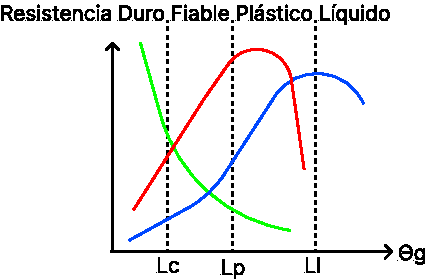
\includegraphics[width=0.5\textwidth]{csa17.pdf}
  \caption{Consistencia del suelo}
  \label{csa17}
\end{figure}
\begin{definition}[Energía potencial]
    Asociada a la posición dentro de un campo de fuerzas
\end{definition}
\begin{example}
    Si una masa de 5kg de agua, es llevada desde un nivel de referencia a 2m por encima de éste, ¿Cuál es su energía potencial?
    \textit{ Sol. }
    \begin{equation}
        E_p = m \cdot g \cdot h
    \end{equation}
    \begin{equation}
        E_c = \frac{1}{2}mv^2
    \end{equation}
    Por lo tanto
    \begin{align*}
        &E_p = 5kg\left(\frac{9.8m}{s^2}\right)\left(2m\right) = 98J\\
        &E_c = \frac{1}{2}mv^2 = \frac{1}{2}(5kg)\left(\frac{0.2m}{s}\right)^2 = 2.5(0.04) = 0.1\\
        &E_c = 0.1kg\cdot \frac{m}{s^2}\cdot m = 0.1J
    \end{align*}
\end{example}
\begin{definition}[Potencial del agua]
    El término potencial puede ser definido como la cantidad  de trabajo realizado o energía almacenada por unidad de masa, volumen o peso de agua, al trasladarla desde un nivel de referencia al punto en cuestión.
\end{definition}
Con base en volumen de agua (sistema mks, jouls/kg)
\begin{equation*}
    \frac{W}{V} = \frac{F \cdot d}{V} =\frac{dinas \cdot cm}{cm^3} =\frac{dinas}{cm^2} = \frac{F}{A} = P
\end{equation*}
Con base en masa de agua (sistema cgs, Erg/gr)
\begin{equation*}
    \frac{W}{m} =\frac{F \cdot d}{m} =\frac{m \cdot g \cdot d}{m} =\frac{Ergios}{gr} =\frac{F \cdot d}{m}
\end{equation*}
Con base en peso
\begin{equation*}
    \frac{W}{P} = \frac{F \cdot d}{g \cdot m} =\frac{m \cdot d \cdot d}{g \cdot m} = cm
\end{equation*}
Para cada una de las fuerzas actuando sobre el agua del suelo, es posible asignar un potencial
\begin{align*}
    &\text{Gravedad}&&\implies&&\text{Potencial gravitacional} \phi g\\
    &\text{Presión}&&\implies&&\text{Potencial de presión} \phi p\\
    &\text{Adsorción}&&\implies&&\text{Potencial matrico} \phi m\\
    &\text{Solutos}&&\implies&&\text{Potencial osmótico} \phi O
\end{align*}
Debido a que el potencial es una cantidad escalar puede ser expresado como una suma algebraica, entonces $\phi_T$ es el potencial total del agua en el suelo:
\begin{equation}
    \phi_T =\phi_g +\phi_p +\phi_m +\phi_o
\end{equation}
El potencial gravitacional, Cuando los puntos bajo análisis están por arriba del nivel de referencia, sus valores serán positivos; si están por abajo de ese nivel de referencia son negativos.

La convención para el potencial de presión, sus valores dentro del suelo, dependerán de la ubicación del nivel freático: por debajo tomará valores positivos y por arriba serán cero.

Con el potencial matrico, en condiciones de saturación tomará valores de 0, y en condiciones de no saturación serán negativos.

Este potencial parcial osmótico, cuando se tenga agua pura será 0 pero tomará valores negativos cuando existan sales

\begin{figure}[h!]
    \centering
      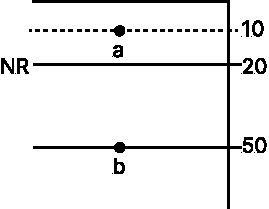
\includegraphics[width=0.5\textwidth]{csa18.pdf}
      \caption{Potencial gravitacional ($\phi g$)}
      \label{csa18}
    \end{figure}
    En la figura \ref{csa18}, $\phi g_{a}=-30cm$ y $\phi g_{b}=10cm$
    \begin{figure}[h!]
    \centering
      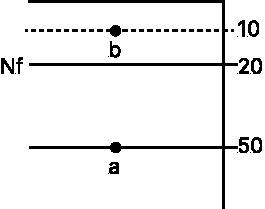
\includegraphics[width=0.5\textwidth]{csa19.pdf}
      \caption{Potencial de presión ($\phi P$)}
      \label{csa19}
    \end{figure}
    En la figura \ref{csa19}, $\phi p_a=30cm$ y $\phi p_b=0cm$
    
    El potencial matrico no aplica los métodos anteriores, mediante tensiómetro. Este es debido a las fuerzas de adsorción del suelo y al fenómeno de capilaridad y cuando existe tiene un valor de cero o negativo (succión), el tensiómetro está en centibares (negativo)
    
    \textbf{El potencial osmótico}
    Este es debido a los suelos disueltos en el agua, y aparece cuando existe una membrana semipermeable como en las relaciones hídricas suelo planta.
    \begin{figure}[h!]
    \centering
      \includegraphics[width=0.5\textwidth]{csa20.pdf}
      \caption{Potencial osmótico}
      \label{csa20}
    \end{figure}
    El potencial osmótico se puede poner de manifiesto si colocamos en un tubo cerrado en forma de U, en una parte agua y en la otra disolución, por ejemplo de agua con azúcar. Ambas se encuentran separadas por una membrana semipermeable.
    
    Esta membrana es permeable para el agua pero impermeable para las moléculas de azúcar.
    
    La disolución atrae agua para diluirse y trata de equiparar las concentraciones a cada lado de la membrana, creándose un potencial osmótico
    
    \subsection{Conductividad hidráulica ($K$) permeabilidad}
    \begin{definition}[Conductividad hidráulica]
        Es la constante de proporcionalidad en la ecuación de Darcy
    \end{definition}
    \begin{equation}
        V =- K\frac{\phi H_2 -\phi H_1}{x_2 - X_1}
        \label{eqcsa1}
    \end{equation}
Es una variable que representa propiedades del medio poroso y del agua
    \begin{equation}
        K =\frac{fd^2\cdot \rho w g}{32\cdot n}
    \end{equation}
    \begin{notation}
        \begin{itemize}
            \item $K$ Conductividad hidráulica $cm/s$
            \item $f$ porosidad total (\%)
            \item $d$ Diámetro promedio de poros ($cm$)
            \item $\rho w$Densidad del agua ($gr/cm^3$)
            \item $g$ Constante gravitacional 0.00981$cm/s^2$
            \item $n$ Viscosidad del agua poises ($gr/(cm\cdot s)$)
        \end{itemize}
    \end{notation}
    Se necesita determinar en campo o laboratorio, suponiendo que $Q=8cm^3/min$ y una área de $10cm^2$, entonces aplicamos la ecuación del gasto sustituida en la ecuación \eqref{eqcsa1}
    \begin{align*}
        \frac{Q}{A} = K\cdot\frac{\phi H_2 -\phi H_1}{X_2 - X_1}\\
        K =\frac{Q\left(X_2 - X_1\right)}{A\left(\phi H_2 -\phi H_1\right)} = \frac{0.6cm}{min}
    \end{align*}
    \begin{figure}[h!]
    \centering
      \includegraphics[width=0.5\textwidth]{csa21.pdf}
      \caption{Prueba de laboratorio del parámetro de carga constante}
      \label{csa21}
    \end{figure}
    Todos los puntos de un sistema suelo en contacto con la atmósfera, poseen potenciales hídricos iguales a cero 
    
    \subsection{Materia orgánica del suelo}
    Materia orgánica (MOS \%), se determina por el método Walkley-black
    
    \begin{table}[h!]
        \centering
        \begin{tabular}{@{}cc@{}}
        \toprule
        \% de M.O.        & Parámetro \\ \midrule
        \textless{}0.9    & Muy bajo  \\
        1-1.9             & Bajo      \\
        2-2.5             & Normal|   \\
        2.6-3.5           & Alto      \\
        \textgreater{}3.6 & Muy alto  \\ \bottomrule
        \end{tabular}
        \caption{Según Rioja, M. 2007}
        \label{tabcsa6}
        \end{table}
    \begin{figure}[h!]
    \centering
      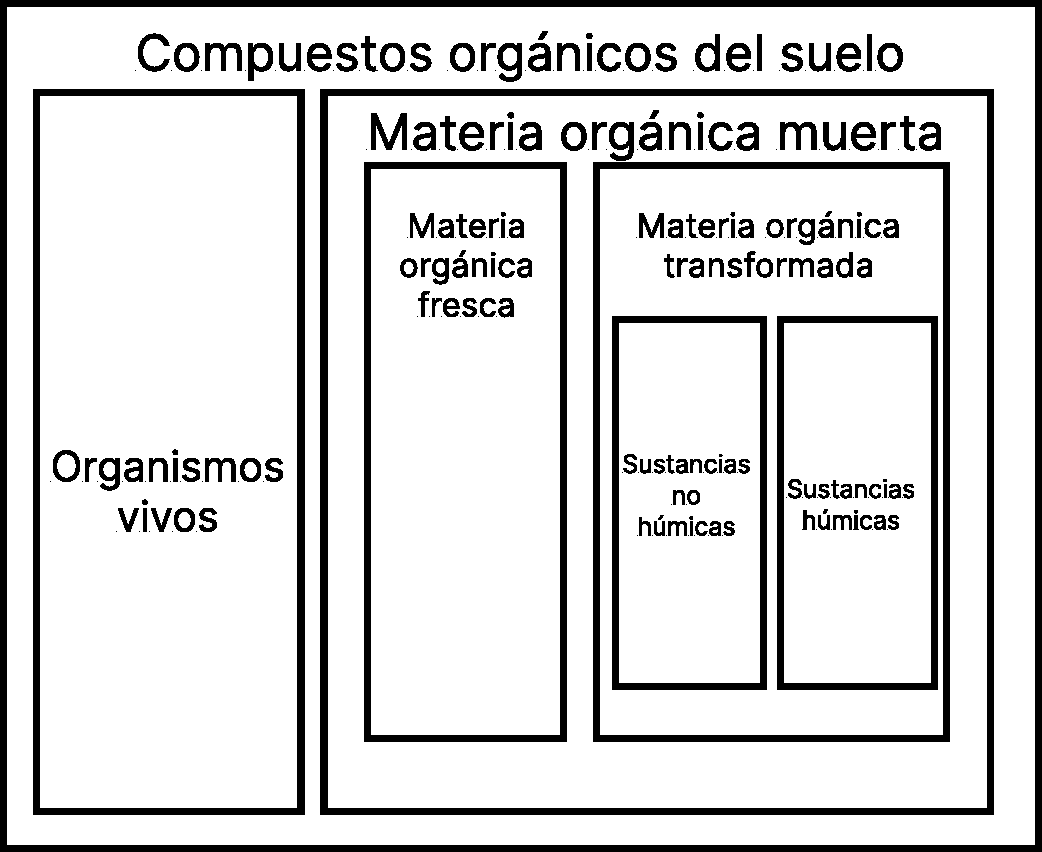
\includegraphics[width=0.5\textwidth]{csa22.pdf}
      \caption{Composición de la materia orgánica del suelo}
      \label{csa22}
    \end{figure}
    \subsection{Materia orgánica}
    Las funciones del suelo se ven directamente afectadas por la cantidad y la calidad de la MO que contiene, por ello la MO es un contribuyente y un indicador de la calidad del suelo.
    \begin{itemize}
        \item Estructuración
        \item Contra el sellado y encostramiento de la superficie del suelo
        \item Porosidad y aireación
        \item Movimiento del agua en el suelo
        \item Capacidad de retención de agua disponible para las plantas
        \item Facilidad de laboreo
        \item Prevención de los procesos erosivos.
    \end{itemize}
    \subsubsection{Propiedades químicas}
    \begin{itemize}
        \item Proceso de intercambio iónico
        \item Capacidad amortiguadora frente a los cambios de pH
        \item Estabilización de nutrientes en forma orgánica (NPS)
        \item Formación de complejos órgano minerales
    \end{itemize}
    \subsubsection{Propiedades biológicas}
    \begin{itemize}
        \item Interviene en la formación del suelo
        \item Reserva de energía metabólica, por las grandes cantidades de C y de nutrientes que contiene
        \item Fuente de macronutriente (NP,S) y micronutrientes (B,Mo), que son liberados en forma progresiva
        \item Estimula e inhibe la actividad enzimática, según los casos
        \item Contiene reguladores del crecimiento de las plantas
        \item Contribuye a la resiliencia de los ecosistemas, al disminuir o inhibir los efectos de las pertubaciones ambientales, u de este modo acelera su recuperación.
    \end{itemize}

    \section{Mecánica de la erosión hídrica}

    \subsection{Definición de erosión y sus agentes}
    \begin{definition}[Erosión]
        Es la pérdida de partículas y nutrientes de la superficie terrestre debido a la acción de los agentes: \begin{itemize}
            \item Agua
            \item Viento
            \item Acción del hombre
        \end{itemize}
    \end{definition}
    La erosión hídrica se produce en tres etapas
    \begin{enumerate}
        \item Desprendimiento de las partículas
        \item Transporte de las partículas
        \item Deposición de partículas del suelo
    \end{enumerate}
    El desprendimiento se debe al impacto de las gotas de lluvia sobre la superficie del suelo con el gasto de su energía cinética, se destruyen los agregados, se produce el salpicamiento de partículas
    
    Los principales factores que controlan la erosión hídrica con el clima (precipitación, humedad, temperatura y evapotranspiración), la cubierta vegetal (intercepción, reducción de la energía cinética de las gotas, morfología de las plantas, y residuos superficiales), la topografía (La erosión se incrementa con más pendiente, determinando la velocidad del agua, capacidad de transporte se incrementa con el incremento de la pendiente, el grado y longitud del pendiente determinan la tasa de escorrentía) y las propiedades del suelo (textura, estructura, porosidad, infiltración, contenido antecedente de humedad, contenido de arcilla, materia orgánica, compactación). Los efectos interactivos de estos factores determinan la magnitud y la tasa de erosión del suelo.
    
    \subsection{Tipos, formas, clases y grados de erosión}
    \subsubsection{Tipos}
    Existe la erosión geológica o erosión inducida o antrópica
    \subsubsection{Formas}
    Las principales formas del suelo son Erosión por salpicadura, Laminar, Por canalillos o surcos, cárcavas, túneles, por corrientes, y grupos especiales de erosión como los pedestales y masa.
    
    \subsubsection{Erosión por salpicamiento}
    El proceso de erosión implica impacto, salpicadura y formación de cráteres. La profundidad de los cráteres es función de la energía de la gota de lluvia que es una función de la velocidad, tamaño y forma de la gota de lluvia; se han desarrollado relaciones matemáticas para estimar las características del cráter de la siguiente manera:
    \begin{equation}
        D = KR\left(\rho V^2\right)^{\frac{1}{3}}
    \end{equation}
    \begin{notation}
    \begin{itemize}
        \item $D=$ Profundidad del cráter en cm
        \item $K=$ Constante
        \item $R=$ Radio de la gota de lluvia (cm)
        \item $\rho=$ Densidad del agua ($gr\cdot cm^{-3}$)
        \item $V=$ Velocidad de la gota de lluvia ($cm\cdot s^{-1}$)
    \end{itemize}
    \end{notation}
    \begin{example}
        \begin{itemize}
            \item K=1
            \item R=0.001cm
            \item $\rho=1gr\cdot cm^{-3}$
            \item $V=981 cm\cdot s^{-1}$
        \end{itemize}
    Calcular el valor de D:
    
    \textit{ Sol. }
        \begin{align*}
            &D =(1)*0.001\left(1\cdot 981^2\right)^{\frac{1}{3}}
            &D = 0.09872cm
        \end{align*}
    \end{example}
    
    El volumen del cráter ($cm^3$) y el área ($cm^2$) son calculados con la siguientes ecuaciones
    \begin{align}
        &V =\frac{1}{3}\pi\cdot D^2\left(\frac{3d^2 + 2D^2}{8D} - D\right)\\
        &A =\pi\left(\frac{d^{2}}{4} + D^2\right)
    \end{align}
    Donde $d$ es el diámetro del cráter (cm). El volumen del cráter basado en la energía cinética ($E_c$) y en la densidad aparente (g $cm^{-3}$) del suelo ($\rho b$) son estimados por la ecuación:
    \begin{equation}
        V =\frac{\rho \cdot d^{\frac{1}{2}\cdot \rho b^{\frac{1}{2}}}}{\rho d + \rho b}\cdot \frac{E_c}{2\phi}
    \end{equation}
    \begin{notation}
        \begin{itemize}
            \item $\rho d$= Densidad de la gota de lluvia
            \item $\phi =$ Resistencia al esfuerzo cortante del suelo
        \end{itemize}
    \end{notation}
    
    \subsubsection{Erosión laminar}
    Es la parte de la escorrentía que fluye entre los canalillos, las partículas son transportadas en la escorrentía que fluye como una lámina delgada; es el tipo más común de erosión del suelo y es una función del desprendimiento de partículas, la intensidad de la lluvia y la pendiente del terreno.
    \begin{equation}
        Di = Ki\cdot I\cdot S
    \end{equation}
    \begin{notation}
        \begin{itemize}
            \item $Di$ Tasa de desprendimiento laminar
            \item $ki$ Tasa de erodabilidad
            \item $I$ Intensidad de la lluvia ($ms^{-1}$)
            \item $S$ Factor pendiente $1.05-0.85\times e^{-4\sin{\theta}}$, donde $\theta$ es el ángulo de la pendiente
        \end{itemize}
    \end{notation}
    \subsubsection{Erosión en canalillos}
    Se produce debido al flujo de concentrado en lugar del flujo laminar poco profundo, el agua se concentra en pequeños canales que erosiona el suelo más rápido que la erosión laminar; la fuerza del flujo y las partículas del suelo que se arrastran a lo largo agrandan los canalillos. Es función de la erodabilidad del suelo, la capacidad de transporte y la fuerza cortante hidráulica
    
    La acción simultánea de la erosión laminar y en canalillos se modela con la ecuación siguiente:
    \begin{equation}
        \frac{\partial  q_s}{\partial x} = Dr + Di
    \end{equation}
    \begin{notation}
        \begin{itemize}
            \item $qs$ Tasa de entrega de sedimentos en canalillos ($kg\cdot m^{-1}\cdot s^{-1}$)
            \item $x$ Longitud de canalillos en m
            \item $Dr$ tasa de desprendimiento en canalillos ($kg m^{-1}\cdot s^{-1}$)
            \item $Di$ Entrega de sedimentos en canalillos ($kg\cdot m^{-2}\cdot s^{-1}$)
        \end{itemize}
    \end{notation}
    $Dr$ es calculado por la ecuación:
    \begin{equation}
        Dr =\alpha\left(T_c -qs\right)
    \end{equation}
    Donde $\alpha= $constante, $T_c$ capacidad de transporte de la escorrentía.
    
    Otra representación matemática del fenómeno es:
    \begin{equation}
                \frac{\partial qs}{\partial x} = K_r\left(\tau -\tau_c\right)\cdot \left(1 -\frac{qs}{T_c}\right)
    \end{equation}
    \begin{notation}
        \begin{itemize}
            \item $Kr$ Erodabilidad en surcos (s $m^{-1}$)
                \begin{equation}
                    \frac{\partial qs}{\partial x} = K_r\left(\tau -\tau_c\right)\cdot \left(1 -\frac{qs}{\tau}\right)
                \end{equation}
            \item $\tau$ Esfuerzo cortante hidráulico (Pa)
            \item $\tau_c$ Esfuerzo cortante crítico (Pa)
            \item $T_c$ Capacidad de transporte de la escorrentía
        \end{itemize}
    \end{notation}
    La ecuación refleja la naturaleza compleja del proceso de erosión.
    \subsubsection{Erosión por cárcavas}
    Crea canales en forma de V o en forma de U, canales de incisión lineal de al menos 0.3m de ancho y 0.3m de profundidad; se forman por el escurrimiento concentrado que converge en los puntos más bajos del campo y se dan en campos ondulados, hacen que la escorrentía se concentre en las corrientes naturales cuando se desplaza hacia abajo en sendas estrechas en forma de caudal canalizado.
    \subsubsection{Erosión por túneles}
    Es común en tierras áridas y semiáridas, suelos con horizontes B altamente erosionables y sódicos pero estables. Las grietas naturales y las madrigueras inician los túneles infiltrando y moviendo capas de subsuelo dispersables. Los túneles o cavidades se expanden hasta el punto en que ya no soportan el peso superficial y se derrumban formando baches y cárcavas.
    \subsection{Erosión hídrica}
    Es el colapso de las paredes de los  cauces a lo largo de arroyos y ríos debido al poder erosivo de la escorrentía de los campos.
    \begin{itemize}
        \item Lo causan el cultivo intensivo,
        \item pastoreo
        \item Tráfico a lo largo de los arroyos
        \item Ausencia de amortiguadores \end{itemize}
    
    
    \subsubsection{Clases cualitativas de erosión hídrica}
    Se tienen las siguientes clases:
    \begin{enumerate}
        \item \textbf{Nula a ligera}: Erosión laminar, los suelos mantienen aún sus características biológicas (materia orgánica) y físicas (estabilidad estructural)
        \item \textbf{Moderada}: Se presentan canalillos y cárcavas aisladas además de erosión laminar. Se observa un descenso importante de la materia orgánica en los suelos así como pérdida de estructura de los mismos
        \item \textbf{Alta y muy alta}: Se presentan cárcavas y surcos en forma significativa. En estos suelos además de haber perdido sus características biológicas y físicas originales se dificulta el paso de la maquinaria debido a la presencia de cárcavas.
    \end{enumerate}
    
    \begin{table}[h!]
            \centering
            \begin{tabular}{@{}cc@{}}
            \toprule
            Clase         & \begin{tabular}[c]{@{}c@{}}Pérdida de suelo\\ (Mg/Ha/año)\end{tabular} \\ \midrule
            Nula a ligera & -10                                                                    \\
            Moderada      & 10-50                                                                  \\
            Alta          & 50-200                                                                 \\
            Muy alta      & 200                                                                    \\ \bottomrule
            \end{tabular}
            \caption{Clases cuantitativas de erosión hídrica}
            \label{tabcsa7}
    \end{table}
    Los límites permisibles se basan en los siguientes aspectos:
    \begin{itemize}
        \item Que las pérdidas sean menores o iguales a la velocidad de formación
        \item Que se mantengan a un nivel que evite la formación de cárcavas
        \item Que permitan mantener una profundidad del suelo que conserve la productividad en el tiempo
    \end{itemize}
    Los límites permisibles son variables en diferentes sitios ya que son una función de la profundidad y del tipo y proceso formador del suelo así como del clima
    
    \subsubsection{Erosividad de las lluvias}
    Se refiere a la capacidad intrínseca de la precipitación para provocar la erosión del suelo. La erosión hídrica no ocurría si las lluvias no fueran erosivas.
    
    Las propiedades de la lluvia que tienen relación con la erosividad son:
    \begin{itemize}
        \item Cantidad
        \item Intensidad
        \item Velocidad terminal de las gotas
        \item Tamaño de las gotas
        \item Distribución del tamaño de las gotas. 
    \end{itemize}
    Recordando que la energía cinética para la tormenta se puede estimar mediante la suma de los valores de la $E_c$ de las gotas, existen varias relaciones matemáticas para relaciones matemáticas para relacionar la intensidad con la energía de la lluvia.
    
    La ecuación universal de pérdida del suelo usa datos sobre la intensidad de la lluvia para calcular la $E_c$ de la siguiente manera:
    \begin{align}
        &E_c = 0.0119 + 0.0873 \log{(i_m)}&& i_m\leq 76mm\cdot h{ -1}\\
        &E_c = 0.283&& i_m\geq 76mm\cdot h^{ - 1}
    \end{align}
    \begin{notation}
        \begin{itemize}
            \item $E_c$ Energía cinética en ($Mj\cdot ha^{-1}\cdot mm^{-1}$ de lluvia)
            \item $I_m$ intensidad de lluvia (mm $h^{-1}$)
        \end{itemize}
    \end{notation}
    % \subsubsection{Intensidad}
    \subsection{Características físicas de la lluvia y el escurrimiento}El análisis parte de los datos de precipitación, esto puede ser
    \begin{itemize}
        \item Precipitación diaria 
        \item Precipitación mensual 
        \item Precipitación anual 
        \item Precipitación media diaria
        \item Precipitación media mensual
        \item Precipitación media anual.
    \end{itemize}
    Forma de las gotas de lluvia:
    \begin{itemize}
        \item Las gotas no tienen forma de lágrima, son pequeñas y casi esféricas
        \item Las gotas más grandes se aplastan en la parte inferior por la resistencia del aire y tienen la apariencia de un pan de hamburguesa
        \item Las gotas grandes tienen una gran cantidad de resistencia al aire, lo que hace que sean inestables
        \item Las gotas muy grandes se dividen por la resistencia del aire. 
    \end{itemize}
    El poder de erosión por impacto de las gotas de lluvia, depende de las siguientes propiedades de las gotas de lluvia:
    \begin{itemize}
        \item Masa
        \item Diámetro o tamaños
        \item Forma (esférica, aplanada)
        \item Velocidad terminal
        \item Distribución del tamaño de gotas
    \end{itemize}
    \subsubsection{Cpalculo de la velocidad límite o terminal (Vt)}
    Similar a la ley de Stokes, cuando una masa de agua cae en un fluido como el aíre por la fuerza de gravedad, está sometido a una fuerza de resistencia o arrastre que se incrementa con la velocidad, la masa alcanzará una velocidad máxima donde las fuerzas de empuje y de arrastre se igualan. Esta velocidad de movimiento constante se llama velocidad límite o velocidad terminal. 
    \begin{equation}
        F_{a_rastre} =frac{1}{2}C\rho AV^2
    \end{equation}
    \begin{notation}
        \begin{itemize}
            \item $\rho$ Densidad del aíre: $1.29kg/m^3$
            \item $A$ Área de la sección transversal (gota esférica) \item $C$ Coeficiente numérico de arrastre=0.5 \item $V$ velocidad (m/s)
        \end{itemize}
    \end{notation}
    La velocidad constante o límite se alcanza cuando la fuerza de arrastre es igual al peso
    \begin{equation}
        mg = \frac{1}{2}C \rho AV
    \end{equation}
    \begin{notation}
        De aquí:
        \begin{itemize}
            \item $V_{terminal}=\sqrt{\frac{2mg}{C\rho A}}$
        \end{itemize}
    \end{notation}
    Si se quiere calcular la $E_c$ de una gota de lluvia lo más correcto sería utilizar la V terminal.
    % \begin{problem}[Utilizando la formula anterior, calcular la velocidad terminal de gotas de lluvia de los siguientes tamaños: 4mm,4.5mm,5mm de radio]
    %     \textit{ Sol. }
    
    %     \begin{align*}
    %         V_{terminal}=\sqrt{\frac{2mg}{C\rho A}}\\
    %         V_{terminal}=\sqrt{\frac{2\cdot \left(m\right)\left(\frac{9.81m}{s^2}\right)}{C\rho A}}\\
            
    %     \end{align*}
    % \end{problem}
    \subsubsection{Fórmulas para obtener la velocidad terminal en función del diámetro de gota}
    Uplinger propuso $V_t$ en m/s y $D$ en cm
    \begin{equation}
        V_t = 4.854 \cdot D \cdot e^{ -0.195D}
    \end{equation}
    Van Dijk propuso:
    \begin{equation}
        V_t = 0.0561D^3 - 0.912D^2 +5.03D- 0.254
    \end{equation}
    Gunn y Kinzer propusieron:
    \begin{equation}
        V_t = 2.9379\ln{(D)} + 4.393
    \end{equation}
    La energía cinética de una gota de lluvia se expresa fácilmente en términos de sus propiedades como:
    \begin{equation}
        E_c = \frac{1}{2}mV^2 = \frac{1}{12}\pi\rho D^3V^2
    \end{equation}
    \begin{notation}
        \begin{itemize}
            \item $\rho$ Densidad del agua
            \item $D$ Diámetro de gota = diámetro de una esfera equivalente
            \item $V$ Velocidad terminal
        \end{itemize}
    \end{notation}
    Por lo tanto, la $E_c$ de un evento de precipitación por unidad de superficie se puede calcular directamente conociendo D la V de cada fota de lluvia. ¿Cómo calcular el número de gotas en una lluvia?
    % NO HAY INVESTIGACIONES SOBRE EROSION HÏDRICA POR EL IMPACTO DE GRANIZO NI NIEVE.
    Sin embargo, estas características de caída no se miden normalmente, sino que se utilizan las relaciones entre $E_c$ y la intensidad de lluvia. Existen dos enfoques principales.
    \begin{itemize}
        \item Ecuaciones de regresión que relacionan empíricamente la energía cinética y la intensidad ($E_c$)
        \item Fórmulas que utilizan modelos de distribución de tamaños de gotas de lluvia.
    \end{itemize}
    Park et al. propusieron la fórmula:
    \begin{equation}
        E_c = 21.1069I^{1.156}\Delta t
    \end{equation}
    La energía cinética se expresa en $j\cdot m^{-2}$, $I$ en $mm\cdot h^{-1}$ y $\Delta t$ en h
    
    \subsubsection{Fórmulas que utilizan modelos de distribución de tamaños de gotas de lluvia}
    Existen dos posibilidades clásicas para utilizar la DGT:
    
    Relacionar el diámetro medio del volumen de gotas (D50) de la precipitaicón y su intensidad. Este D50 se supone que es un diámetro efectivo capaz de reproducir las propiedades de todo el conjunto de gotas de lluvia.
    
    Considerar un modelo de DTG de la precipitaicón en lugar del D50.
    
    Ambas formas necesitan el conocimiento de velocidad terminal de la gota, pero mientras que el uso del diámetro medio de la gota necesita saber solamente una velocidad única V (D50), fácil de deducir de tablas publicadas, el de un modelo completo de DTG necesita introducir el espectro completo de velocidades.
    
    Usando las relaciones D50 de la literatura, la energía cinétrica se puede expresar como:
    \begin{equation}
        E_c = \frac{I\Delta t}{2}V^2 \cdot D_{50}
    \end{equation}
    
    \begin{notation}
        \begin{itemize}
            \item $V(Dso)$ es la velocidad terminal en $m/s$ de una gota de lluvia de diámetro D50 en $mm$, se tiene cuatro fórmulas conocidas para obtener D50.
        \end{itemize}
    \end{notation}
    Laws \& Parson, basándose en sus propios datos y en los de leyes, propusieron la relación:
    \begin{equation}
        D_{50}= 1.238I^{0.182}
    \end{equation}
    Atlas en base a datos de Marshall y Palmer, D50 lo expresa como:
    \begin{equation}
        D_{50} = 921 I^{0.21}
    \end{equation}
    Brandt basado en sus propios datos, prpuso la relación:
    \begin{equation}
        D_{50}= 1.416I^{0.123}
    \end{equation}
    Villis basado en daos de dos ciclones tropicales recolectaods po una lluvia óptica con un espectómetro propuso:
    \begin{equation}
        D_{50} = 0.97I^{0.158}
    \end{equation}
    \subsubsection{Datos para la distribución del tamaño de gota (Disdrómetor)}
    En las útlimas décadas, la medida de las características de las gotas de lluvia se ha facilitado por el desarrollo del \textbf{Disdrómetro} y espectrómetro de lluvia óptica.
    
    Este dispositivo se basa en un principio electromecánico y determina el tamaño (D) de las fotas de lluvia a partir de la medición de la fuerza vertical aplicada por las gotas que caen sobre un transductor.
    \begin{itemize}
        \item La señal suministrada se procesa para obtener D en 25 clases de diámetros igualmente espaciadas de 0.2mm
        \item La superficie de muestreo, S, es de $50cm^2$ y la gama de diámetros de gotas medibles es de 0.2mm hasta 5.2mm
        \item El espectro de tamaño de gotas de lluvia se registra cada 30s
    \end{itemize}
    Algunos aspectos importantes son que en un evento de lluvia es un conjunto de gotas de lluvia de diversos tamaños golpeanod a la superficie receptora; la distribución del tamaño de las gotas determinan: volumen e intensidad; La erosividad de un evento de lluvia depende de la carga de ener´gia que lleva en relación con la distribución del tamaño de la gota y la velocidad de impacto. La caracterización de las tormentas de lluvia al expresar el rango completo de la distribución del tamaño de las gotas proporciona una descripción más completa de la precipitación que la cantidad de lluvia y/o su intensidad.
    
    Las lluvias intensas, con una alta tasa de lluvia por unidad de área y tiempo, son causadas por gotas de mayor diámetro, o más gotas con diámetro menor recibidas por unidad de tiempo por unidad de área.
    El tamaño de gota de las tormentas naturales varía considerablemente desd e0.1mm hasta un límite superior de aproximadamente 6mm.

    Los datos sobre la medición del tamaño de las gotas se expresan generalmente de dos maneras:
    \begin{itemize}
        \item Rango de distribución del tamaño de gota
        \item El tamaño medio de la gota (D50)
    \end{itemize}
    
    Cuanto mayor es la cantidad de lluvia por evento y cuando mayor es la intensidad, ayor es el tamaño mediano de la gota.
    
    El diámetro mediano de la gota (D50) oscila entre 2.34 y 4.86mm con un amedia de 3.42mm. Otros observaron el diámetro mediano de la gota de 2.1mm a 5.2mm.
    \subsection{Métodos para estimar las pérdidas de suelo}
    Los datos experimentales sobre la cantidad de suelo erosionado son requeridos para:
    \begin{itemize}
        \item Evaluar la magnitud o gravedad de la erosión y ss efectos sobre la productividad del suelo 
        \item Probar la aplicabilidad de algunos modelos matemáticos para reducir la erosión del suelo
        \item Diseñar y establecer prácticas de control de la erosión
        \item Evaluar los procesos de sedimentación en áreas de deposición
        \item Determinar los efectos de la erosión en la contaminación del agua
    \end{itemize}
    \subsubsection{Estacas o clavos con rondanas}
    La cuantificación de las pérdidas mediante el método de clavos se gace a través de la siguiente fórmula:
    \begin{equation}
        P = H \cdot A \cdot D_a
    \end{equation}
    \begin{notation}
    \begin{itemize}
        \item $P$ pérdida de suelo
        \item $H$ altura de la lámina pérdida
        \item $A$ Área medida
        \item $D_a$ Densidad aparente
    \end{itemize}
\end{notation}
    \subsubsection{Parcelas de escurrimiento}
    Existen tres tipos de parcelas para determinr la erosión:
    \begin{itemize}
        \item Microparcelas de 0.5 a 2.0m
        \item Parcelas medianas o ISLE 4 por 22.1m
        \item Parecñas grandes o cuencas hidrográficas de al menos $100m^2$
    \end{itemize}
    \begin{figure}[h!]
    \centering
      \includegraphics[width=0.5\textwidth]{csa23.jpg}
      \caption{Las parcelas de escorrentía brindan información para la sistematización de tierras, la construcción de terrazas y la identificación de estrategias de manejo para el control de la erosión hídrica.}
      \label{csa23}
    \end{figure}
    \subsubsection{Recipientes para salpicadura}
    Sirven para cuantificar la erosión por salpicadura
    \begin{figure}[h!]
    \centering
      \includegraphics[width=0.5\textwidth]{csa24.png}
      \caption{Mcdición de ia erosión por salpicadura mediante embudos\cite{pelaez2003metodos}}
      \label{csa24}
    \end{figure}
    \subsubsection{estación de aforo y colectores}
    Una estación de puente como en la figura, se mide el área transversal del flujo,
    velocidad con el molinete y se puede obtener un caudal y medir cuánto suelo se está perdiendo en 
    laboratorio para tener la sedimentación. 
    \begin{figure}[h!]
    \centering
      \includegraphics[width=0.5\textwidth]{csa25.jpg}
      \caption{Estación de aforo}
      \label{csa25}
    \end{figure}
    \begin{definition}[Modelo]
        Es una representación simplificada de un sistema real que puede:
        \begin{itemize}
            \item Reproducir la realidad
            \item Simplificar la realidad
            \item Identificar procesos
            \item Estudiar procesos
            \item Pronosticar resultados
            \item Pronosticar procesos
        \end{itemize}
    \end{definition}
    En el desarrollo de la ciencia se han diseñado y aplicado modelos durante siglos en diferentes disciplinas debido a que:
    \begin{itemize}
        \item Es más fácil trabajar con los modelos que con los sistemas reales
        \item En ocasiones los sitesmas son demasiados grandes y complejos
        \item Limitación de recursos humanos y económicos
        \item Imposibilidad de experimentar en algunos sistemas
        \item Para pronosticar resulttados en situaciónes y condiciones específicas
        \item PLantear nuevas hipótesis
        \item Orientar la investifación hacia los puntos más críticos
        \item Tramsferir conocimeientos generados sobre diversas prácticas en diferentes regiones
        \item Para diseñar su manejo a través de la simulación.
    \end{itemize}
    El advenimiento de herramientas tecnológicas como la teledetección y los SIG ha aumentado considerablemente la utilidad d elos modelos de erosión del suelo
    El acoplamiento de SIG y la teledetección con modelos empíricos u nasados en procesos d eerosión del suelo ha mejorado su capacidad predictiva. El SIG almacena la base de datos esencial necesarioa como insumo para modelar la erosión y la elanoración de mapas de las áreas afectadas por la erosión.
    \subsubsection{Modelos de simulación para erosión}
    Existe una amplia gama de modelos para simular el transporte de sedimentos y el transporte de contaminantes asociados. EN general, los modelos se dividen en tres categorías principales:
    \begin{enumerate}
        \item Empíricos o estadísticos / métricos
        \item Conceptuales
        \item Basados en la Física o con base física.
    \end{enumerate}
    Los modelos son generalmente nombrados por sus siglas:
    \begin{itemize}
        \item WEEP Water erosion prediction project (physical)
        \item CREAMS Chemical runoff and erosion from agricultural management systems (physical)
        \item USLE Universal soil loss equation (empirical)
        \item RUSLE Revised Universal SOil Loss Equation (empirical)
        \item EUROSEM European soil loss model
        \item SWAT Soil and Water Assessment tool
        \item EPIC Erosion Productivity Impact Calculator.
    \end{itemize}
    \subsubsection{Eciación universal de pérdidas de suelo}
    \begin{equation}
        A = RKLSCP
    \end{equation}
    \begin{notation}
        \begin{itemize}
            \item $A=$ Pérdidas de selo en (t/Ha)
            \item $R=$ Erosividad de la lluvia ($Mj\cdot  mm\cdot  Ha^{-1}\cdot hr^{-1}$)
            \item $K=$ Erodabilida ddel suelo ($t\cdot ha\cdot  hr\cdot  Mj^{-1}\cdot mm^{-1}\cdot Ha^{-1}$)
            \item $L=$ Longitud de la pendiente (adim)
            \item $S=$ Pendiente, grado de (adim)
            \item $C=$ Manejo (cobertura vegetal) (adim)
            \item $P=$ Prácticas mecánicas (adim)
            \item Factor activo (R) y pasivo (K), los factores LSCP son llamados secundarios.
        \end{itemize}
    \end{notation}
    $A=RK$ cuando el terreno presenta las condiciones estándar que son:
    \begin{itemize}
        \item L= 22.13m de longitud de pendiente
        \item 9\% de pendiente o inclinación del terreno
        \item Condición de terreno desnudo con barbecho contínuo
        \item Laboreo en el sentido de la pendiente.
    \end{itemize}
    se define como:
    \begin{equation}
        R = E_c\cdot l_{30} = EI_{30}
    \end{equation}
    \begin{notation}
        \begin{itemize}
            \item Índice de erosividad para un evento ($MK\cdot mm / (Ha\cdot hr)$)
            \item $E_c$ energía cinética total de la lluvia (MJ/Ha)
            \item $I_{30}$ intensidad mácima de la lluvia en 30 min (mm/Hr)
        \end{itemize}
    \end{notation}
    Wischmeier y colaboradores propusieron una ecuación para calcular la $E_c$ de la lluvia a partir de su intensidad
    \begin{equation}
        E_c = A + B\left(\log{l} \right)
    \end{equation}
    A y B puden tomar diferentes valores numéricos, según las unidades que s utilicen para la intensdida de la lluvia (Pulgadas/hr, cm/hr, mm/hr). La versión más utilizada es:
    \begin{equation}
        E_{ci} = 0.119 + 0.0873 \log{l_i} 
    \end{equation}
    \begin{notation}
        \begin{itemize}
            \item $l_i$ es la intensdiad de la lluvia, en el intervalo u, expresada en $mm/hr$
            \item $E_{c1}$ es la energía cinética para el intervalo de tiempo i, en $MJ/(Ha\cdot mm)$
            \item $t_i$ es el tiempo de intervalo en minuts
            \item $p_i$ es la cantidad de lluvia en el intervalo de tiempo $i$ en mm
        \end{itemize}
    \end{notation}
    Para calcular la energía cinética de una tormenta se aplica la siguiente ecuación
    \begin{equation}
        E_c =\sum_{i = l}^n E_{ci}p_i
    \end{equation}
    \begin{notation}
        \begin{itemize}
            \item $E_c$ es la energía cinética total para el evento en MJ/Ha
            \item $n$ es el número de intervalos con diferente intensidad durante el mismo evento.
            \item $Ec_i$ y $p_i$ ya fueron definidos
        \end{itemize}
    \end{notation}
    Con todo lo anterior la expresión algebráica de R es:
    \begin{equation}
        R=\sum_{j= l}^m (EI_{30})j
    \end{equation}
    \begin{notation}
        \begin{itemize}
            \item $R=$ Es el factor de erosividad de la lluvia o índice de erosividad anual de Wischmeier, expresado en Mj/ha/año
            \item $E=$ Enrgía cinética total para el evento j
            \item $m=$ Número de eventos durante el año.
        \end{itemize}
    \end{notation}
        
    \begin{problem}[Calcular el índice $El_{30}$ para una tormenta con las características]
    
    \end{problem}
    \begin{align*}
        &l_i =p_i\left(\frac{60}{t_i}\right) = 1.25\left(\frac{60min/hr}{20min }\right)\\
        &\left(\frac{1.25m}{h}\right)=3.75mm/h
    \end{align*}
    A continuación se clacula la energía de un mm de lluvia a esa intensidad en una Ha, columna seis del cuadro,
    \begin{equation*}
        E_{c_1}=0.119+ 0.0873 \log{l_i}= 0.119 + 0.0873 \log{3.75} = 0.169 MJ / (ha\cdot mm) 
    \end{equation*}
    Pero como la lluvia caída en ese lapso fue de 1.25 mm entonces
    \begin{equation*}
        E = \left(E_{ci}\right)\left(p_i\right) = 0.169 \cdot 1.25= 0.211 MJ / ha
    \end{equation*}
    sol
    Para calcular la energía de la tormenta, hay que calcular la intensidad de la lluvia en cada ``transecto de intensidad''. Así para el primer lapso de tiempo con tormenta, de las 4:00 a las 4:20 el regístro indica que llovió 1.25mm, así que la intensidad en ese caso es:
    \begin{table}[h!]
        \centering
        \begin{tabular}{@{}ccccccc@{}}
        \toprule
        Tiempo &
          \begin{tabular}[c]{@{}c@{}}Lámina\\ mm\end{tabular} &
          \begin{tabular}[c]{@{}c@{}}Duración\\ min\end{tabular} &
          \begin{tabular}[c]{@{}c@{}}Cantidad\\ mm\end{tabular} &
          \begin{tabular}[c]{@{}c@{}}Intensidad\\ mm/hr\end{tabular} &
          Ec/mm MJ/ha*mm &
          \begin{tabular}[c]{@{}c@{}}$E_c$ total\\ MJ/ha\end{tabular} \\ \midrule
        4:00 & 0.00  & -  & 0.00  & -     & -     & -     \\
        4:20 & 1.25  & 20 & 1.25  & 3.75  & 0.169 & 0.211 \\
        4.27 & 3.00  & 7  & 1.75  & 15.00 & 0.222 & 0.388 \\
        4:36 & 8.75  & 9  & 5.75  & 38.33 & 0.257 & 1.478 \\
        4:50 & 26.25 & 14 & 17.50 & 75.00 & 0.283 & 4.953 \\
        4:57 & 30.00 & 7  & 3.75  & 32.14 & 0.251 & 0.941 \\
        5:05 & 31.25 & 8  & 1.25  & 9.38  & 0.204 & 0.255 \\ \bottomrule
        \end{tabular}
        \caption{Tabla del problema}
        \label{tabcsa8}
    \end{table}
    Calculando de la misma manera para todos los lapsos y al sumar los datos se obtiene la energía cinética total de la tormenta:
    
    Se puede observar que la intensidad máxima se presentó entre las 4:36 y las 4:50 y se mantuvo durante 14 minutos, sin embargo para el $I_{30}$ se requieren 30 minutos, esta condición se cumple desde las 4:27 a las 4:57, lapso en el que llovieron 27mm, (5.75+17.5+3.75). Entonces para una hora se tienen 54mm
    \begin{equation*}
        El_{30}=\left(\frac{8.226MJ}{Ha}\right)\left(\frac{54mm}{hr}\right) = 444.2\cdot\frac{Mj\cdot mm}{Ha\cdot Hr}
    \end{equation*}
    \subsubsection{EL factor K}
    Puede ser evaluado en lotes experimentales, si se resuelve la ecuación
    \begin{equation}
        K = \frac{A}{RLSCP}
    \end{equation}
    para condiciones no estándar de L,S,C,P. De otra manera para condiciones estándar:
    \begin{equation}
        K = \frac{A}{R}
    \end{equation}
    Sin embargo el procedimiento experimental es costoso y tardado, por lo que se propuso el uso de un Nomograma para obtener el valor de $K$.
    
    Datos necesarios para utilizar el nomograma:
    \begin{itemize}
        \item Porcentaje de limos (0.002-0.05mm) y de arenas muy finas (0.05-0.10mm)
        \item Porcentaje de arena (0.1-2.0mm)
        \item Contenido de M.O. en \%
        \item Estructura
        \item Permeabilidad 
    \end{itemize}
    Los tres primeros se determinan en laboratorio y los dos últimos en campo.
    \begin{figure}[h!]
    \centering
      \includegraphics[width=0.5\textwidth]{csa26.png}
      \caption{Cídogs de estructura del suelo de USLE}
      \label{csa26}
    \end{figure}
    \begin{table}[h!]
        \centering
        \begin{tabular}{@{}cc@{}}
        \toprule
        \begin{tabular}[c]{@{}c@{}}Código\\ USLE\end{tabular} & \begin{tabular}[c]{@{}c@{}}Categoría de\\ Permeabilidad\end{tabular} \\ \midrule
        1 & Rápida (más de $12.7 cm\cdot hr^{-1}$)             \\
        2 & Moderada a rápida (6.3 a $12.7 cm\cdot hr^{-1}$)   \\
        3 & Moderada (entre $2 y 6.3 cm\cdot hr^{-1}$)         \\
        4 & Lenta a moderada (entre $0.5 a 2 cm\cdot hr^{-1}$) \\
        5 & Lenta (entre $0.13 a 0.5 cm\cdot hr^{-1}$)         \\
        6 & Muy lenta (menor a $0.13cm\cdot hr^{-1}$)          \\ \bottomrule
        \end{tabular}
        \caption{Categoría de Permeabilidad}
        \label{tabcsa9}
    \end{table}
    \begin{figure}[h!]
    \centering
      \includegraphics[width=0.5\textwidth]{csa27.jpg}
      \caption{ Nomograma del factor K (Figueroa et al., 1991)}
      \label{csa27}
    \end{figure}
    \begin{equation}
        K = \frac{0.00021 \cdot \left(M^{1.14}\right) \cdot \left(12 -\alpha\right) + 3.25\cdot \left(b - 2\right) + 3.3\left(10^{ -3}\right)\left(c- 3\right)}{100}
    \end{equation}
    \begin{notation}
        \begin{itemize}
            \item M= \% de limo de arena muy fina multiplicado por el 100\% de arcilla
            \item $M$ es el prámetro de tamaño de partícula
            \item $a$ es el \$ del contenido de materia orgánica
            \item $b$ es el código de la estructura del suelo (1-4)
            \item $c$ es la permeabilidad del perdil (conductividad hidráulica saturada) 1-6
        \end{itemize}
    \end{notation}
    \subsubsection{Factor de pendiente LS}
    Representa el factor de la topografía, L se define como la distancia desde el punto de origen del escurrimiento hasta:
    \begin{itemize}
        \item Donde la pendiente disminuye dando lugar a la sedimentación
        \item Donde el agua entra a un canal.
    \end{itemize}
    Para L se utiliza
    \begin{equation}
        L =\left(\frac{x}{22.13}\right)^m
    \end{equation}
    \begin{notation}
        \begin{itemize}
            \item $x$ es la longitud de la pendiente, en metros
            \item $m$ es exponente que depende del grado de pendiente
        \end{itemize}
    \end{notation}
    La magnitud del exponente (m) varía como se indíca a continuación:
    \begin{itemize}
        \item $m=0.5$ si la pendiente del terreno es mayor de 5\%
        \item $m= 0.4$ para pendientes entre 3\% y 5\%
        \item $m= 0.3$ para mendeintes entre 1\% y 3\%
        \item $m=0.2 $si la pendiente es menor a 1\%
    \end{itemize}
    $S$ se utiliza con la siguiente ecuación
    \begin{equation}
        S = 0.065 +0.045s + 0.0065s^2
    \end{equation}
    \begin{notation}
        \begin{itemize}
            \item $S$ factor de gradiente de pendiente, para usar en la EUPS
            \item $s$ pendiente del terreno, en porcentaje
        \end{itemize}
        Uniendo $L$ y $S$ se obtiene el valor conjunto del factor de topografía (LS)
    \end{notation}
    \begin{equation}
        LS=\left(\frac{x}{22.13}\right)^m\left(0.065 + 0.045s + 0.0065s^2\right)
    \end{equation}
    \begin{example}
        Calcular el factor topográfico de un terreno con pendeinte constante de 7\% en una longitud de 78m
    \end{example}
    \textit{ Sol. }
    $x=78m;\, m=0.5;\, s=7\%$ por lo tanto
    \begin{equation*}
        LS=\left(\frac{78}{22.13}\right)^{0.5}\left(0.065 + 0.045\times 7 + 0.0065\times 7^2\right) = 1.31
    \end{equation*}
    Lo cuál indirectamente nos permite predecir la pérdida de suelo debido a la pendiente y en consecuencia la influencia del riego.
    
    \subsubsection{Factor c de manejo y cobertura}
    \begin{table}[h!]
        \centering
        \begin{tabular}{@{}cc@{}}
        \toprule
        Cultivos herbáceos        & 0.3  \\ \midrule
        Plantaciones de olivar    & 0.5  \\
        Viñedos                   & 0.6  \\
        Cereales en tierras bajas & 0.35 \\
        Cereales en tierras altas & 0.43 \\
        Hortalizas                & 0.25 \\
        Almendras                 & 0.45 \\
        Prados                    & 0.15 \\
        Plátanos                  & 0.05 \\
        Pastizales arbolados      & 0.2  \\
        \begin{tabular}[c]{@{}c@{}}Regadíos extensivos en\\ zonas semiáridas\end{tabular} & 0.3 \\ \bottomrule
        \end{tabular}
        \caption{Los valores de $C$ fluctúan de 0 para un terreno completamente protegido a 1.0 para un terreno totalmente desprotegido.}
        \label{tabcsa10}
    \end{table}
    \subsubsection{Factor P método de control de la erosión}
    El factor es la proporción de la pérdida de suelo que se presenta cuando se hace uso de una práctica específica, en comparación con la pérdida de suelo cuando se cultiva en laderas sin práctica de conservación alguna.
    
    Los métodos de control incluidos en este factor son generalmente surcado al contorno, terráceo o cultivo en fajas.  
    \begin{table}[h!]
        \centering
        \begin{tabular}{@{}lllll@{}}
        \toprule
        \multirow{2}{*}{\begin{tabular}[c]{@{}l@{}}Pendiente\\ \%\end{tabular}} &
          \multirow{2}{*}{Cultivo a nivel} &
          \multirow{2}{*}{Cultivo en fajas} &
          \multicolumn{2}{l}{Cultivo en terrazas} \\
              &     &      & a    & b    \\ \midrule
        1-2   & 0.6 & 0.3  & 0.12 & 0.05 \\
        3-8   & 0.5 & 0.25 & 0.1  & 0.05 \\
        9-12  & 0.6 & 0.3  & 0.12 & 0.05 \\
        13-16 & 0.8 & 0.35 & 0.14 & 0.05 \\
        17-20 & 0.8 & 0.4  & 016  & 0.06 \\
        21-25 & 0.9 & 0.45 & 0.18 & 0.06 \\ \bottomrule
        \end{tabular}
        \caption{a= terrazas de desagüe cubiertas con césped, $b=$ terrazas de infiltración con contrapendiente}
        \label{tabcsa11}
    \end{table}
    \begin{example}
        Considérese el caso de un terreno con las siguientes características:
        \begin{itemize}
            \item Pendiente del 6\%
            \item Suelos de textura media con profundidad de 70cm sobre roca
            \item 60m de longitud en el sentido de la pendiente
            \item Ubicación del sitio en Lagos de Moreno Jalisco
            \item Cultivado con maíz bajo condiciones de temporal y surcos al contorno.
        \end{itemize}
        Estime las pérdidas de suelo para estas condiciones.
    \end{example}
    \textit{ Sol. }
    \begin{align*}
        &R= 5000MJ / ha / año\\
        &K = 0.02\\
        &L =\text{ Se calcula con }L=\left(\frac{60}{22.13}\right)^{0.5} = 1.65\\
        &S = 0.065 + 0.045s + 0.0065s^2\\
        &S = 0.065 + 0.045(6) + 0.0065(6)^2 = 0.569\\
        &C = 0.51\\
        &P_1 = 0.5
    \end{align*}
    Entonces la pérdida de suelo estimada es:
    \begin{equation*}
        A = RKLSCP = 5000 \cdot 0.02 \cdot 1.65 \cdot 0.569 \cdot 0.51 \cdot 0.5 = 23.94 \frac{t}{ha\cdot año}
    \end{equation*}
    Una vez estimada la pérdida de suelo con la EUPS, se compara con la pérdida permisible y de resulta más alta, se procede a seleccionar una o varias modificaciones en cuanto al manejo, cambio de cultivo o prácticas por realizar. Las modificaciones se hacen sobre LSCP, mientras que R y K se consideran fijos.
    
    \subsubsection{Utilidad de la ecuación universal de pérdidas de suelo}
    Erosión hídrica potencial:
    \begin{equation}
        A = R \cdot K \cdot L \cdot S
    \end{equation}
    Es la susceptibilidad que tiene una zona o región o erosionarse por sus características de clima, suelo y relieve.
    
    Es la erosión que existiría en un determinado lugar, sin acción del hombre y sin la cubierta vegetal protectora.
    
    Las bondades de aplicar este modelo es:
    \begin{itemize}
        \item Es el modelo empírico más utilizado en todo el mundo para estimar la pérdida de suelo
        \item Simplifica los procesos de erosión del suelo. Fue diseñado específicamente para predecir la pérdida de suelo de los suelos cultivados bajo características específicas
        \item Proporciona una estimación anual promedio a largo plazo de la pérdida de suelo a partir de pequeñas parcelas o segmentos de campo con dimensiones definidas
        \item Es ventajoso sobre modelos sofisticados porque es simple, fácil de usar, y no requiere numerosos parámetros de entrada o extensos conjuntos de datos para la predicción
        \item Los parámetros de entrada o extensos conjuntos de datos para la predicción
        \item Los parámetros se estiman a partir de simples gráficos y ecuaciones
        \item Estima las pérdidas de suelo para terrenos diferentes a los agrícolas.
    \end{itemize}
    Sus limitaciones:
    \begin{itemize}
        \item Escorrentía, nutrientes y pérdida de suelos de cuencas o áreas a escala de campo
        \item Pérdida del suelo por evento o diaria
        \item Variabilidad de la pérdida de suelo de tormenta a tormenta
        \item Erosión laminar, en canalillos, en cárcabas y en ríos por separado
        \item Procesos de flujo concentrado de canalización de flujo y deposición de sedimentosProcesos detallados por ejemplo, desprendimiento, transporte y deposición
        \item Tamaño, densidad, área superficial y otras características de los sedimentos, que son importantes para estimar su potencial de adsorción y transporte de sustancias químicas.
    \end{itemize}
    
    \subsection{USLE modificado (MUSLE)}
    Mientras que USLE predice el rendimiento del sedimento basado en la precipitación, MUSLE lo predice utilizando el factor de escorrentía. Esta modificación permite el uso de USLE para predecir la pérdida de sedimentos en base a tormentas
    \begin{equation}
            \text{Sedimentos} = 11.8\left(Q\cdot q_p\cdot A\right)^{0.56} \cdot K \cdot C \cdot P \cdot LS \cdot FFRG
    \end{equation}
    \begin{notation}
        \begin{itemize}
            \item Sedimentos= producción de sedimentos por evento de tormenta (MG)
            \item Q = Escurrimiento superficial (m)
            \item $q_p$ escurrimiento pico o máximo
            \item A Área de la unidad de respuesta hidrológica ($m^2$)
        \end{itemize}
    \end{notation}
    El FFRG es estimado con:
    \begin{equation}
        FFRG = e^{ -0.053 \cdot Rocas}
    \end{equation}
    Donde las rocas es el porcentaje de roca sen la capa más alta de suelo.
    \begin{itemize}
        \item Es más completo y detallado que el USLE
        \item Incluye más valores de EI
        \item Incorpora procesos en suelo como cambios en el contenido de humedad
        \item Incorpora información sobre efectos de la temperatura y de la humedad sobre la descomposición de residuos
        \item Calcula los calores de C a partir de subfactores
        \item Calcula los valores de P basándose en la longitud de pendiente y la inclinación, la deposición del suelo, la infiltración del suelo y las condiciones de cubierta y rugosidad
        \item Considera el factor de cobertura (CC) que representa la cubierta vegetal
        \item Considera la cobertura superficial (SC) por cantidad de residuos de mantillo que queda en la superficie
        \item Considera el factor de rugosidad superficial.
    \end{itemize}
    Un sistema hidrológico que produce escurrimientos se conjugan o interrelacionan la entrada, el funcionamiento y su salida
    \begin{equation}
        y(t) =h(t)\Psi x(t)
    \end{equation}
    \begin{notation}
        \begin{itemize}
            \item $\psi=$ indica combinación
            \item $h(t)=$ Función de operación
            \item $x(t)=$ función de entrada
            \item $y(t)=$ Función de salida
        \end{itemize}
    \end{notation}
    Cuando se conocen dos de las tres funciones citadas, se puede obtener la desconocida:
    \begin{itemize}
        \item Si la desconocida es la salida, el problema es de predicción
        \item Si se desconoce el funcionamiento el problema es de calibración o identificación
        \item Si se desconoce la entrada, el problema es de detección
    \end{itemize}
    La fórmula del método racional es:
    \begin{equation}
        Q=FU \cdot C \cdot I \cdot A
    \end{equation}
    \begin{notation}
        \begin{itemize}
            \item $Q=$ es el gasto máximo o pico
            \item $C=$ coeficiente de escurrimiento que es adimensional
            \item $I=$ la intensidad de lluvia
            \item $A=$ es el área del sistema
            \item $FU=$ factor de unidades
        \end{itemize}
    \end{notation}
    Características de la lluvia (intensidad o lámina)
    
    Características del sistema: Coeficiente de escurrimiento, el tiempo de concentración y área
    
    Es el tiempo que trascurre entre el inicio de la lluvia y el establecimiento del gasto de equilibrio donde la cantidad de agua que está entrando por precipitación es igual a la cantidad de agua que está saliendo como escurrimiento.
    
    El escurrimiento sea superficial, subsuperficial o subterránea en la salida de una cuenca llamado ``boquilla'', la representación gráfica del gasto en función del tiempo es el hidrográma
    \begin{equation}
        Q=0.0278CIA
    \end{equation}
    \begin{notation}
        \begin{itemize}
            \item $I=$ intensidad media de la lluvia para una duración igual al $t_c$ de la cuenca, en mm/h
            \item $A=$ área de la cuenca, en $km^2$
        \end{itemize}
    \end{notation}
    \begin{equation}
        Qp=\frac{CLA}{360}
    \end{equation}
    \begin{notation}
        \begin{itemize}
            \item $L$ lluvia máxima en 24 horas para un $Tr$ dado (mm)
            \item $A$ área de drenaje
            \item $Q_p=$ escurrimiento máximo ($m^3/s$)
        \end{itemize}
    \end{notation}
    Es el tiempo en años para que aparezca un evento de la misma magnitud
    
    Cálculo de $t_c$ según Kirpich
    \begin{equation}
        t_c=\left(\frac{0.56L_c}{H}\right)0.325
    \end{equation}
    \begin{notation}
        \begin{itemize}
            \item $t_c$ Tiempo de concentración en horas
            \item $L_c$ Longitud del cauce principal (km)
            \item $H$ Desnivel entre extremos de cuace principal (m)
        \end{itemize}
    \end{notation}
    \begin{table}[h!]
        \centering
        \begin{tabular}{@{}cccc@{}}
        \toprule
        \multirow{2}{*}{Pendientes} &
          \multicolumn{3}{c}{Textura de suelos} \\
         &
          Arenoso &
          \begin{tabular}[c]{@{}c@{}}Limo-\\ Arcilloso\end{tabular} &
          Arcilloso \\ \midrule
        \begin{tabular}[c]{@{}c@{}}Bosques\\ 0-5\\ 5-10\\ 10-30\end{tabular} &
          \begin{tabular}[c]{@{}c@{}}0.10\\ 0.25\\ 0.30\end{tabular} &
          \begin{tabular}[c]{@{}c@{}}0.30\\ 0.35\\ 0.50\end{tabular} &
          \begin{tabular}[c]{@{}c@{}}0.40\\ 0.50\\ 0.60\end{tabular} \\
        \begin{tabular}[c]{@{}c@{}}Pasturas\\ 0-5\\ 5-10\\ 10-30\end{tabular} &
          \begin{tabular}[c]{@{}c@{}}0.10\\ 0.15\\ 0.20\end{tabular} &
          \begin{tabular}[c]{@{}c@{}}0.30\\ 0.35\\ 0.10\end{tabular} &
          \begin{tabular}[c]{@{}c@{}}0.40\\ 0.55\\ 0.60\end{tabular} \\
        \begin{tabular}[c]{@{}c@{}}Tierras de cultivo\\ 0-5\\ 5-10\\ 10-30\end{tabular} &
          \begin{tabular}[c]{@{}c@{}}0.30\\ 0.40\\ 0.50\end{tabular} &
          \begin{tabular}[c]{@{}c@{}}0.50\\ 0.60\\ 0.70\end{tabular} &
          \begin{tabular}[c]{@{}c@{}}0.60\\ 0.70\\ 0.80\end{tabular} \\ \bottomrule
        \end{tabular}
        \caption{Coeficiente de escurrimiento C, cuencas rurales}
        \label{tabcsa12}
    \end{table}
 \subsubsection{Curvas intensidad duración y frecuencia}
    Las curvas IDF corresponden a la representación gráfica de la relación que existe entre la intensidad y la duración, asociado a la frecuencia o periodo de retorno de la precipitación. La relación intensidad duración frecuencia de precipitaciones extremas es ampliamente usada para estimar las avenidas de diseño en los sitios donde se construirán las obras hidráulicas. Aunque en estudios recientes se ha encontrado que la variabilidad de la precipitaciones están cuestionado las curvas IDF
    
    La fórmula que relaciona simultáneamente las tres variables es:
    \begin{equation}
        i = \frac{k \cdot T^m_r}{(d+ c)^n}
    \end{equation}
    \begin{notation}
        \begin{itemize}
            \item $i=$ intensidad de precipitación (mm/h)
            \item $T=$ periodo de retorno (años)
            \item $d=$ duración (minutos)
            \item $k,m,n,c=$ parámetros que se calculan a partir de los datos, mediante un análisis de correlación lineal múltiple, d puede ser $t_c$
    \end{itemize}
    \end{notation}
    \begin{example}
        Para una cuenca se tienen los siguientes datos: $k=615, m=0.18, d=tc=11.6min, c=5, n=0.685, A=125ha, C=0.46, Tr=25$ años. Aplicando el método racional encuentre Q máximo o pico.
    
        \textit{ Sol. }
        \begin{align*}
            &Q = \frac{C \cdot I \cdot A}{360}\\
            &I= \frac{k\cdot Tr^m}{(d+c)^n}\\
            &I=\frac{615\times 25^{0.18}}{(11.6+5)^{0.685}}=160.22m/h\\
            &Q=\frac{0.46\times 160.22\times 125}{36} ==25.59\frac{m^3}{s}  
        \end{align*}
    \end{example}
    Se basa en el concepto de que en toda tormenta, la lluvia en exceso Q es siempre menor o igual a la lámina de precipitación P. De manera similar, después de que se inició el escurrimiento, la lámina de agua retenida en la cuenca F es menor o igual a la retención potencial máxima S. Existe una cantidad de precipitación la (denominada sustracción inicial antes del encharcamiento) para la cual no se produce escorrentía superficial. Por lo tanto el escurrimiento potencial es $P-la$; la hipótesis del método de SCS consiste en que las relaciones entre las cantidades reales y las potenciales son constantes, y estas son:
    
    \begin{notation}
        \begin{itemize}
            \item $P=$ Precipitación
            \item $Q=$ Lluvia en exceso (siempre Q<P)
            \item $S=$ Retención potencial máxima
            \item $F=$ Lámina de agua retenida en el sistema (después de que se inició el escurrimiento $F\leq S$)
            \item $ia=$ Precipitación inicial antes de encharcamiento = cero escorrentía superficial. Por lo tanto el escurrimiento potencial es $P-ia$
        \end{itemize}
    \end{notation}
    La siguiente ecuación describe las condiciones en las que no se produce ninguna abstracción inicial
    \begin{equation}
        \frac{F}{S}=\frac{Q}{P}
    \end{equation}
    \begin{notation}
        \begin{itemize}
            \item $F=P-Q$ retención real después de que comienza la escorrentía
            \item $Q$ escorrentía real
            \item $S$ retención máxima potencial después de que comienza la escorrentía
            \item $P$ escorrentía máxima potencial (es decir, precipitación total si no hay una abstracción inicial)
        \end{itemize}
    \end{notation}
    \subsubsection{Deducción de la fórmula}
    \begin{align*}
        &\frac{P-Q}{S}=\frac{Q}{P}\\
        &P(P-Q)=SQ\\
        &PP-PQ=SQ\\ 
        &p^2=SQ+PQ\\ 
        &p^2=Q(S+P)\\
        &Q=\frac{p^2}{S+P}\\
        &Q=\frac{(P-ia)^2}{(S+P-ia)}\\
        &Q=\frac{(P-0.2S)^2}{(S+P-0.2S)}\\
        &Q=\frac{(P-0.2S)^2}{(P+0.8S)}
    \end{align*}
    \subsubsection{Obtención de S}
    $S$ se relaciona con las condiciones del suelo y el tipo de cobertura superficial a través de las CN:
    \begin{equation}
        S = \frac{25400}{CN}- 254
    \end{equation}
    
    $S$ es la diferencia potencial máxima entre P y Q a la hora que se inicia la tormenta y representa proporcionalmente la pérdida de escorrentía por infiltración, intercepción y almacenamiento superficial.
    Los parámetros del método USDA o del número de curva son el tipo de suelo, condición hidrológica,el uso y manejo del suelo.
    \subsubsection{Deducción de la fórmula}
    \begin{align*}
        &\frac{P-Q}{S}=\frac{Q}{P}\\
        &P(P-Q)=SQ\\
        &PP-PQ=SQ\\ 
        &p^2=SQ+PQ\\ 
        &p^2=Q(S+P)\\
        &Q=\frac{p^2}{S+P}\\
        &Q=\frac{(P-ia)^2}{(S+P-ia)}\\
        &Q=\frac{(P-0.2S)^2}{(S+P-0.2S)}\\
        &Q=\frac{(P-0.2S)^2}{(P+0.8S)}
    \end{align*}
    
    \subsection{Método USDA o del número de curva}
    \subsubsection{Tipo de suelo}
    \begin{itemize}
        \item Tipo A: Bajo potencial de escurrimiento (arenosos)
        \item Tipo B: Moderadamente bajo potencial de escurrimiento
        \item Tipo C: Moderadamente alto
        \item Tipo D: Alto (arcillosos)
    \end{itemize}
    Condición hidrológica
    \begin{itemize}
        \item Buena cv>75\%
        \item Regular cv enter 50 y 75\%
        \item Mala cv<50\%
    \end{itemize}
    \begin{table}[h!]
        \centering
        \begin{tabular}{@{}ccccccc@{}}
        \toprule
        \multicolumn{3}{c}{Cobertura}                      & \multicolumn{4}{c}{Tipo de suelo} \\ \midrule
        Uso de suelo & tratamiento & Condición hidrológica & A      & B      & C      & D      \\
        Rastrojo        & Texto       & mala                 & 66     & 70     & 80     & 90     \\ \bottomrule
        \end{tabular}
        \caption{Todos los factores expresados}
        \label{tabcsa13}
        \end{table}
    \begin{align}
        Q = \frac{(P - 0.2S)^2}{P + 0.8S}&&S = \frac{25400}{CN} - 254
    \end{align}
    \begin{notation}
        \begin{itemize}
            \item $Q$ Gasto
            \item $P$ Precipitación en mm
            \item $S$ Potencial máximo de retención de humedad
            \item $CN$ Valores de tablas
        \end{itemize}
    \end{notation}
    \begin{table}[h!]
        \centering
        \begin{tabular}{@{}cc@{}}
        \toprule
        \begin{tabular}[c]{@{}c@{}}Condición de\\ humedad\\ antecedente\end{tabular} &
          \begin{tabular}[c]{@{}c@{}}Precipitación acumulada\\ de los cinco días previos\\ al evento en (mm)\end{tabular} \\ \midrule
        I  & 0-12.7              \\
        II & 12.7-38.1           \\
        II & P\textgreater{}38.1 \\ \bottomrule
        \end{tabular}
        \caption{Condición de humedad antecedente como función de la precipitación}
        \label{tabcsa14}
    \end{table}
    En caso de que el valor de la tabla \ref{tabcsa14}, sea I o III se usa la segunda tabla.
    \begin{table}[h!]
        \centering
        \begin{tabular}{@{}lll@{}}
        CN10      & \multicolumn{2}{l}{CN correspondientes} \\
        condición & Condición I        & Condición II       \\
        100       & 100                & 100                \\
        95        & 87                 & 98                 \\
        90        & 78                 & 96                 \\
        85        & 70                 & 94                 \\
        80        & 63                 & 91                 \\
        75        & 57                 & 88                 \\
        70        & 51                 & 85                 \\
        65        & 45                 & 82                 \\
        60        & 40                 & 78                 \\
        55        & 35                 & 74                 \\
        50        & 31                 & 70                 \\
        45        & 26                 & 65                 \\
        40        & 22                 & 60                 \\
        35        & 18                 & 55                 \\
        30        & 15                 & 50                 \\
        25        & 12                 & 43                 \\
        20        & 9                  & 37                 \\
        15        & 6                  & 30                
        \end{tabular}
        \caption{Curvas numéricas para condiciones antecedentes de humedad del suelo, Húmeda (III) y seca (I) a partir de las condiciones de humedad intermedia (II)}
        \label{tabcsa15}
    \end{table}
    
    Ecuaciones para pasar de un NC con condición de humedad antecedente II a uno con condición I y III
    \begin{align}
        &CN(I) = \frac{4.2\times CN(II)}{10 -0.58\times CN(II)}\\
        &CN(III) = \frac{23\times CN(II)}{10 + 0.13\times CN(II)}
    \end{align}
    \begin{example}
        Si se tiene que NC=74 pero se quiere obtener el valor para la condición seca y la húmeda es decir I y III
        \textit{ Sol. }
        \begin{align*}
            &CN(I) = \frac{4.2\times 74}{10 -0.058\times 74} = 54.4\\
            &CN(III) = \frac{23\times 74}{10 + 0.13\times 74} = 86.7
        \end{align*}
    \end{example}
    \begin{example}
        Se tiene un área de bosque ralo, condición hidrológica mala, grupo de suelos B y precipitación de 106.5mm
        \textit{ Sol. }
        \begin{align*}
            Q = \frac{\left(106.5 - 0.2(130.86)\right)^2}{106.5 + 0.8 \cdot 130.86} = 0.56mm\\
            S = \frac{25400}{66} - 254 = 130.86
        \end{align*}
    \end{example}
    \subsubsection{Aplicación de qp y Q en MUSLE}
    MUSLE tiene la capacidad de predecir la erosión hídrica utilizando el factor de escorrentía. Esta modificación permite el uso de USLE para predecir la pérdida en base en tormentas
    \begin{itemize}
        \item Eventos futuros
        \item Probabilidad de ocurrencia
        \item Son necesarios datos
        \item Variables aleatorias
        \item Población y muestra
        \item Análisis con el histograma
        \item Histograma y funciones de densidad y distribución de probabilidades.
    \end{itemize}
    Se usan funciones de probabilidad más utilizadas en hidrología como la Normal, Log-normal, Exponencial, Gamma, Gumbel, Log-Pearson, etc.
    
    \begin{definition}[Periodo de retorno T]
        Es el tiempo promedio que transcurre entre la ocurrencia de ese evento y la próxima ocurrencia de ese evento con la misma magnitud
    \end{definition}
    Está ligado a la probabilidad de una distribución probabilística mediante la ecuación:
    \begin{equation}
        T = \frac{1}{P(x\geq x_i)} =\frac{1}{1 -P(x\leq x_i)}
    \end{equation}
    \begin{notation}
        \begin{itemize}
            \item $P(X\geq x)$ probabilidad de que la variable aleatoria x tome un valor mayor x
            \item $T$ periodo de retorno en años
        \end{itemize}
    \end{notation}
    Fórmula de aplicación de Weibull
    \begin{equation}
        P(X\geq x) = \frac{1}{T} = \frac{m}{n +1}
    \end{equation}
    \begin{notation}
        \begin{itemize}
            \item $P(X\geq x)=$ probabilidad de que la variable aleatoria x tome un valor $\geq x$
            \item $T=$ periodo de retorno en años
            \item $n=$ Número totales de datos
            \item $m=$ Número de orden, ordenados los datos de mayor a menor.
        \end{itemize}
    \end{notation}
    Para adoptar el período de retorno a utilizar en el diseño de una obra, es necesario considerar la relación existente entre la probabilidad de excedencia de un evento, la vida útil de la estructura y el riesgo de falla admisible, dependiendo de este ultimo, de factores económicos, sociales, técnicos y otros. El riesgo de falla admisible en función del perido de retorno y vida útil de la obra está dado por:
    \begin{equation}
        R = 1 - 1\left(1 - \frac{1}{T}\right)^n
    \end{equation}
    Donde el máximo es el menor y el mínimo es el mayor riesgo.
    
    \section{Métodos y técnicas para el control de la erosión}
    Los métodos y técnicas son diversos agrupados en tres grupos:
    \begin{itemize}
        \item Prácticas mecánicas
        \item Prácticas agronómicas
        \item Prácticas vegetativas.
    \end{itemize}
    
    \begin{definition}[Prácticas mecánicas]
        Implican el movimiento de suelo con el propósito de evitar las pérdidas de suelo y agua por escorrentía y aumentar la humedad del terreno. Controlan el transporte de las partículas, pero no propician la agregación por ejemplo terrazas, drenajes, canales de desviación, canales de desagüe, zanjas desviadoras, zanjas de infiltración, zanjas trinchera, tinas ciegas, franjas al contorno y cauces empastados.
    \end{definition}
    
    \begin{definition}[Prácticas agronómicas]
        Manejo del terreno para mejorar las propiedades del suelo, tienden a reducir la densidad aparente, incrementar la capacidad de infiltración, disminuir el escurrimiento y conservar la humedad. Actúan principalmente contra la desagregación del suelo. Por ejemplo la labranza cero, mínima, de conservación, en franjas, al contorno, surcos al contorno, subsoleo, agroforestería, encalados, incorporación de MO, composta y Mulching.
    \end{definition}
    
    \begin{definition}[Prácticas vegetativas]
        Desarrollo de plantas, cultivos o vegetación natural para mejorar la capacidad productiva y disminuir la erosión, por ejemplo la rotación de cultivos, cultivos en fajas, asociados o policultivos, cobertera, sistemas agroforestales, y cortinas rompevientos.
    \end{definition}
    
    \begin{definition}[Terrazas]
        Son terraplenes formados entre los bordos de tierra, o la combinación de bordos y canales, construidos en sentido perpendicular a la pendiente del terreno.
    \end{definition}
    Sirven para reducir la erosión del suelo, aumentar la infiltración del agua en el suelo para que esta pueda ser utilizada por los cultivos; disminuir el volumen de escurrimiento que llega aguas abajo; desalojar las excedencias de agua superficial a velocidades no erosivas; reducir el contenido de sedimentos en las aguas de escorrentía y acondicionar los terrenos para las labores agrícolas.
    
    Se pueden clasificar según la condición de escurrimiento ó el tipo de sección transversal
    
    De la condición de escurrimiento:
    \begin{enumerate}
        \item Terrazas con declive: Área con precipitación anual mayor de 800mm o donde los suelos propician la acumulación de agua que es necesario desalojar hacia una salida
        \item Terrazas a nivel: Áreas con precipitaciones menores de 800mm anuales, o donde los suelos son profundos, con buena permeabilidad y capaces de retener toda el agua de lluvia.
    \end{enumerate}
    La sección transversal está formada de un bordo y un canal. La sección consta de tres pendientes laterales conocidas como pendiente de corte, pendiente frontal y contrapendiente
    \begin{figure}[h!]
    \centering
      \includegraphics[width=0.5\textwidth]{csa28.png}
      \caption{Esquema de una terraza}
      \label{csa28}
    \end{figure}
    El espaciamiento consta de dos distancias:
    \begin{itemize}
        \item Intervalo vertical (IV) diferencia de nivel entre terrazas (m)
        \item Intervalo horizontal (IH) distancia horizontal entre terrazas (m)
    \end{itemize}
    De acuerdo a la sección transversal se tienen terrazas de base ancha, bancales, canal de zingg y de base angosta.
    \begin{figure}[h!]
    \centering
      \includegraphics[width=0.5\textwidth]{csa29.png}
      \caption{Clasificación}
      \label{csa29}
    \end{figure}
    En la \textbf{Base ancha}, se aplican en terrenos erosionables con pendientes mayores de 8\%, resistentes a la erosión con límite de 12\% o terrenos con pasto, con límite de 15\%.
    \begin{align}
        IV = \frac{S +4}{10}&&IV = \frac{S + 6}{10}&& IH = \frac{IV}{S} \cdot 100
    \end{align}
    En el \textbf{Bancal}, se utilizan en áreas con topografía muy accidentada, zonas con alto riesgo de erosión, zonas donde hay posibilidades de regar los cultivos, pendientes que no excedan más del 50\% y suelos con horizonte A o capa arable con relativa profundidad
    \begin{align}
        W = \frac{200\cdot d}{S}&& IV = \frac{S \cdot W}{100 - S}
    \end{align}
    \begin{notation}
        \begin{itemize}
            \item W= ancho de la terraza en metros
            \item d= profundidad máxima del corte (m)
            \item S= pendiente del terreno (\%)
        \end{itemize}
    \end{notation}
    En el \textbf{Canal amplio o zingg}, se usan cuando hay pendientes suaves (0.5-5\%) preferentemente, se requiere un suelo profundo que proporciones capacidad de almacenamiento de la humedad, efectos productivos mínimos por efecto de los cortes y el espaciamiento depende del área necesaria de escurrimiento y de captación.
    
    En la terraza de \textbf{Base angosta}, sirven para captar agua de lluvia y al desagüe de los escurrimientos superficiales
    \begin{align}
        IV =\left(2 + \frac{P}{304}(0.305)\right)&&IH =\left(\frac{IV}{P}(100)\right)
    \end{align}
    \subsubsection{Criterios de diseño}
    \begin{example}
        Terraza de base angosta: Canal de sección triangular, terreno de textura media, pendiente del 14\% área de escurrimiento de la terraza de 1.09 ha ($27.21\times 400m$) y es de uso agrícola
        \textit{ Sol. }
        
        Calcular el volumen de escurrimiento, fórmula racional:
        \begin{equation*}
            Q_p=0.028*0.72*1.09=0.109872m^3/s
        \end{equation*}
        
        Obtención de la velocidad máxima permisible: como son suelos erodables con una longitud de terrazas mayor a 150m y con vegetación de tablas V=0.225m/s, de acuerdo al material del canal.
        Calcular el área de la sección transversal con la fórmula:
        \begin{equation*}
            A= \frac{Q}{V} =\frac{0.1099}{0.225}=0.4884m^2
        \end{equation*}
    
    Determinación del a sección del canal que permita manejar el volumen de agua a una velocidad adecuada, para ello se tiene que realizar los siguiente:
    \begin{itemize}
        \item Cálculo del radio hidráulico (de acuerdo al tipo de canal), para poder obtener $r^{2/3}$ se desea un canal triangular con taludes 10:1, entonces se apliaca:
        \begin{equation*}
            d = \sqrt{\frac{A}{Z}} = \sqrt{\frac{0.40884}{10}}== 0.22m
        \end{equation*}
        Para el perímetro mojado es: $P=2d \sqrt{z^2+1}=2(0.22)\sqrt{100+1}=4.42m$
    
        Con los valores de A y P se aplica $r=\frac{A}{P}=\frac{0.4884}{4.42}=0.11$
        
        Se obtiene la relación hidráulica: $r^{2/3}=0.11^{2/3}=0.229$
        \item Con el valor de la pendiente permisible se obtiene $S^{1/2}$
        Si la pendiente permisible es de 0.35\% entonces $S=0.0035\implies S^{1/2}=0.0035^{1/2}=0.05916$
        \item Valor del coeficiente de rugosidad n de acuerdo a las condiciones del cauce (tablas), $n=0.06$
        \item Con los valores se procede aplicar la fórmula de Manning para encontrar la velocidad
        \begin{equation}
            V = \frac{r^{\frac{2}{3}}S^{\frac{1}{2}}}{n} = \frac{0.229\times 0.05916}{0.06} = 0.2257m/\frac{0.2257m}{s}
        \end{equation}
    \end{itemize}
    La velocidad permisible es de 0.255 m/s, como la velocidad obtenida es igual a la velocidad máxima permisible, los valores son correctos Para comprobar que las dimensiones del canal son las adecuadas se utiliza:
    \begin{equation*}
        Q= AV = 0.4884 \cdot 0.2257 = 0.1102 \frac{m^3}{s}
    \end{equation*}
    El valor es mayor que el volumen máximo a conducir obtenido con la fórmula racional ($0.1099m^3/s$) pero la aproximación es suficiente para definir las características del canal con fines prácticos.
    \end{example}
    Son zanjas rectángualres de dos metros de longitud, 0.5m de base y 0.5m de profundidad y construidas siguiendo las curvas de nivel. Conservan la humedad para los árboles o las plantaciones forestales.
    \begin{itemize}
        \item Sirven para controlar la erosión en laderas con cobertura vegetal deteriorada que requieren repoblación
        \item Almacenar agua en el suelo para el uso de las plantas o de los cultivos forestales
        \item Recargar de mantos acuíferos 
        \item Reducir la velocidad del escurrimiento superficial 
        \item y Actuar como brechas cortafuegos
    \end{itemize}
    Localización y requisitos para su empleo: En regiones áridas o semiáridas donde la Precipitación no es muy alta, en laderas sin vegetación de una cuenca hidrográfica para hacer una reforestación y para el desarrollo de huertos en terrenos de ladera.
    \begin{enumerate}
        \item Escurrimiento total con el método de CN
        \item 50\% del escurrimiento total
        \item Área tributaria necesaria para una tina de cm por 0.5m por 0.5m, es decir $0.5m^3$
        \item Distancia vertical entre tinas en la misma dirección (dt)
        \item Distancia vertical entre hieras de tinas (dl)
    \end{enumerate}
    \begin{figure}[h!]
    \centering
      \includegraphics[width=0.5\textwidth]{csa30.png}
      \caption{Ejemplo de distribución de tinas ciegas en un terreno}
      \label{csa30}
    \end{figure}
    \begin{example}
        Considere la siguiente información para el diseño de tinas ciegas:
        \begin{itemize}
            \item Lluvia máxima en 24 horas = 68.5mm
            \item 290 ha de bosque con poca cobertura (condición hidrológica mala)
            \item 271 ha de pastizales muy pastoreados (condición hidrológica regular)
            \item Lluvia en los cinco  días previos de 42.5mm
        \end{itemize}
        \textit{ Sol. }
    
        Escurrimiento total del método de la curva numérica:
        \begin{equation*}
            S = \frac{25400}{CNA} - 254
        \end{equation*}
        Con los valores ajustados de la curva numérica se calcula el potencial máximo de retención (S)
        \begin{table}[h!]
            \centering
            \begin{tabular}{@{}cccc@{}}
            \toprule
            Zona & CN & CHA & CNA  \\ \midrule
            1    & 66 & III & 82.6 \\
            2    & 66 & III & 84.4 \\ \bottomrule
            \end{tabular}
            \caption{Donde S1=53.5mm y S2=46.95mm}
            \label{tabcsa16}
            \end{table}
    \begin{equation*}
        A = \frac{(P - 0.2S)^2}{P + 0.8S}
    \end{equation*}
    Con estos valores se pondera el escurrimiento medio, tal como se muestra en el recuadro siguiente:
    \begin{table}[h!]
        \centering
        \begin{tabular}{@{}ccccccc@{}}
        \toprule
        Zona & Área (ha) & S(mm) & PP(mm) & Q(mm) & AQ(mm)   & Q(mm) \\ \midrule
        1    & 290       & 53.5  & 68.5   & 30.01 & 8702.9   & 30.46 \\
        2    & 2701      & 46.95 & 68.5   & 30.94 & 8384.74  &       \\
             & 561       &       &        &       & 17087.64 &       \\ \bottomrule
        \end{tabular}
        \caption{Escurrimiento medio}
        \label{tabcsa17}
        \end{table}
        \begin{equation*}
            Q = \frac{Qt}{At} = \frac{17087.64}{561Ha} = 30.46mm
        \end{equation*}
    EL 50\% del escurrimiento total es:
    \begin{equation*}
        \frac{Q}{2} = \frac{30.46mm}{2} = 15.23mm
    \end{equation*}
    Escurrimiento a captar de 15.23mm
    
    Área tributaria de escurrimiento:
    \begin{equation}
        \text{Volumen }m^3=\text{Lámina de escurrimiento (m)}\times \text{Área tributaria (m)}
    \end{equation}
    Entonces, despejando la ecuación anterior:
    \begin{equation*}
        \text{Área tributaria }(m^2)= \frac{0.5m^3}{0.01523m}= 32.83m^2
    \end{equation*}
    
    La distancia entre tinas de la misma dirección:
    \begin{equation*}
        dt = \frac{32.84m^2}{2m} = 16.42m
    \end{equation*}
    $dt$ distancia entre tinas en la misma dirección,
    
    Distancia vertical entre línea de tinas:
    
    Por su colocación eb ek terreno, la distancia entre líneas de tinas (dl) será igual a:
    \begin{equation*}
        dl =\frac{dt}{2} = \frac{16.42}{2} = 8.21
    \end{equation*}
    
    Por último del número de tinas por hectárea:
    \begin{itemize}
        \item En 100m entran 25 tinas
        \item El espaciamiento entre líneas de tinas es de  8.21m
        \item En 100m se tienen 100m/8.21=12.18 líneas
        \item El número de tinas por ha es de $25\times 12=300$ tinas
    \end{itemize}   
    \end{example}


    \section{Obras hidráulicas para control de azolves}
    \begin{definition}[Carcavas]
        Zanjas causadas por la erosión hídrica, que siguen la máxima pendiente del terreno que constituyen un cauce donde se concentra y corre el agua proveniente de las lluvias. El agua que corre por la cárcava arrastra gran cantidad de partículas de suelo producto de la erosión
    \end{definition}
    \begin{enumerate}
        \item El agua de escurrimiento desciende por la superficie del suelo
        \item Encuentro de irregularidades en el relieve del terreno
        \item El agua se concentra formando pequeños surcos
        \item Los surcos se juntan y forman un canal mayor y por tanto se mueve una masa de agua mayor
        \item La masa de agua mayor provoca el agrandamiento horizontal y vertical formándose la cárcava
        \item Aparece la erosión remontante que da una mayor longitud a la cárcava
    \end{enumerate}
    Los agentes causales son los cambios de uso del suelo, uso inadecuado de laderas, lluvias de alta intensidad, hábito subterráneo de roedores, prácticas inadecuadas de laboreo, ruptura de obras aguas arriba y aprovechamiento forestal.
    
    Las partes y características de una cárcava son:
    \begin{enumerate}
        \item Cabeza
        \item Paredes
        \item Fondo
        \item Profundidad
        \item Pendiente
        \item Longitud o desarrollo.
    \end{enumerate}
    % Las \textbf{Carcavas discontinuas} Son cárcavas que aparecen de manera aislada y
    Según los perfiles transversales: en V, cóncava o en U, cuadrado o en cajón, escalonado e irregular.
    \begin{figure}[h!]
    \centering
      \includegraphics[width=0.5\textwidth]{csa31.jpg}
      \caption{Perfiles de una cárcava}
      \label{csa31}
    \end{figure}
    \begin{itemize}
        \item Cárcava pequeña: Si la profundidad es menor a un metro
        \item Cárcava mediana: Sí la profundidad es de uno a cinco metros
        \item Si la profundidad es mayor de cinco metros.
    \end{itemize}
    Los daños son que tiene un arrastre de suelo fértil y pérdida de materia orgánica, azolvamiento de obras hidráulicas, reducen el área cultivable, afectan el tránsito de maquinaria o vehículos, pérdida de insumos agrícolas, disminución de productividad, y restringen el uso de la tierra.
    
    La rehabilitación y control de cárcavas considera dos principios básicos, la rehabilitación parcial y total.
    
    La rehabilitación parcial consiste en:
    \begin{itemize}
        \item No llegar a recuperar el estado original de la cárcava
        \item El problema de degradación persiste
        \item Se ocasionan gastos inútiles, tiempo y esfuerzo
        \item No controla la erosión remontante (origen de la cárcava)
    \end{itemize}
    La rehabilitación total (cara definitiva)
    \begin{itemize}
        \item Considera la rehabilitación del sistema hidráulico
        \item Utiliza estructuras permanentes de control
        \item Crea nuevas condiciones hidráulicas para el escurrimiento
        \item Controla la erosión remontante.
    \end{itemize}
    Los principios básicos de control de cárcavas son:
    \begin{enumerate}
        \item Mejorar las condiciones de la zona desde donde vierte el agua a la cárcava para reducir la escorrentía (por ejemplo aumentando la cobertura vegetal)
        \item Desviar, toda o parte de la escorrentía que entra en la cárcava
        \item Estabilizar la cárcava mediante medidas estructurales (casi siempre por fiques de retención) o revegetación.
    \end{enumerate}
    Los aspectos para atender en el control de una cárcava
    \begin{enumerate}
        \item Longitud origen de la cárcava \begin{enumerate}
            \item Etapa conocida como cabeceo de la cárcava
            \item Controla el crecimiento longitudinal de la cárcava
            \item Control de la erosión remontante
        \end{enumerate}
        \item Ancho (estabilización de taludes) \begin{enumerate}
            \item Estabilizar taludes en ambas márgenes de la cárcava
            \item Se controla yr educe el escurrimiento superficial lateral
            \item Se controla el desarrollo de cárcavas laterales
        \end{enumerate}
        \item Profundidad \begin{enumerate}
            \item Evitar que la cárcava profundice
            \item Control del escurrimiento superficial en el fondo
        \end{enumerate}
        \item Caracterización física del suelo: Se determinan las características físicas del suelo a fin de conocer su comportamiento al momento de cimentar la obra.
    \end{enumerate}
    \subsubsection{Obtención del escurrimiento máximo en una cárcava con la fórmula de manning}
    Para la obtención del gasto es necesario tener el área hidráulica de la sección transversal y velocidad del agua en la cárcava
    \begin{equation}
        Q = A \cdot V
    \end{equation}
    \begin{enumerate}
        \item Ubicar los niveles laterales del agua en la cárcava utilizando las huellas máximas por medio de dos estacas
        \item Colocar una cuerda para determinar el nivel que tendría el agua en la cárcava al alcanzar estos niveles
        \item Localizar en el fondo de la cárcava las zonas con pendientes homogéneas, colocando estacas para delimitarlas
        \item Utilizando dos estadales y colocándolos de manera vertical en los puntos marcados con las estacas (ver la burbuja centrada) formar áreas transversales parciales tomando las alturas
        \item Con una cinta métrica tomar la anchura de las secciones parciales y formar figuras regulares generalmente rectángulos, triángulos y trapecios
        \item Obtener el área de cada figura y cada sección parcial
        \item Sumando las áreas parciales obtener el área transversal total de la cárcava.
    \end{enumerate}
    \subsubsection{Procedimiento para obtener el perímetro mojado y radio hidráulico}
    \begin{enumerate}
        \item Utilizando las estacas colocadas para la obtención de las áreas parciales, medir la distancia entre cada par de ellas con una cinta métrica recorriendo de manera transversal la cárcava
        \item En cada medición se debe colocar la cinta ajustada a la superficie del fondo de la cárcava
        \item Sumar las distancias parciales desde la primera estaca lateral hasta la última, y de esta manera obtener el perímetro mojado (P) \begin{equation}
            R = \frac{A}{P}
        \end{equation}
    \end{enumerate}
    \subsubsection{Procedimiento para la obtención de la pendiente}
    \begin{enumerate}
        \item Utilizando un clisímetro y un estadal y ubicándose el observador en una zona plana obtener la altura del clisímetro por medio de un estadal
        \item Ubicar una estaca de cinco metros aguas arriba y otra cinco metros aguas debajo de los puntos geométricos que ubican la sección transversal de la cárcava
        \item Ubíquese el observador con el clisímetro en el punto aguas arriba y un estadal en el punto aguas abajo
        \item Enfoque con el clisímetro la altura del aparato medida, moviendo la palanca de desplazamiento del clisímetro hasta que la burbuja que se visualiza con el clisímetro queda centrada
        \item Registre el dato pendiente en \% marcada en el clisímetro.
    \end{enumerate}
    
    \subsection{Presas de control}
    Las presas de control de asolve de acuerdo a los materiales emplados para su construcción y la vida útil de estos se clasifican en permanentes y temporales.
    \begin{enumerate}
        \item Estructuras permanentes \begin{enumerate}
            \item Presas de mampostería hidráulica
            \item Presas de mampostería seca
            \item Presas de gaviones
            \item Presas de muro vivo
        \end{enumerate}
        \item Estructura temporales \begin{enumerate}
            \item Presas de costales
            \item Presas de ramas y palos
            \item Presas de muro vivo
        \end{enumerate}
    \end{enumerate}
    Las presas de control de azolves de acuerdo a su funcionamiento en relación a la retención del agua se clasifican en filtrantes y no filtrantes:
    \begin{enumerate}
        \item No filtrantes \begin{enumerate}
            \item Presas de mampostería hidráulica
            \item Presas de mampostería seca
        \end{enumerate}
        \item Filtrantes \begin{enumerate}
            \item Presas de costales
            \item Presas de ramas y morillos o troncos
            \item Presas de muro vivo
        \end{enumerate}
    \end{enumerate}
    Desde el punto de vista metodológico, se pueden clasificar en dos grandes grupos: Diseño empírico o hidráulico.
    
    Tiene especificaciones generales del diseño para cualquier tipo de presa:
    \begin{itemize}
        \item Altura
        \item Espaciamiento 
        \item Vertedor 
        \item delantal
    \end{itemize}
    \subsubsection{Especificaciones generales}
    Su altura: Temporales, alrededor de 1m y permanentes de 5m o más (es necesario el diseño para lograr su estabilidad)
    
    Espaciamiento: Depende de la pendiente, la altura y la cantidad de sedimentos a retener, se tienen dos alternativas: cabeza-pie ó doble cabeza-pie.
    \begin{equation}
        E=\frac{H}{Pc}\times 100
    \end{equation}
    \begin{notation}
    \begin{itemize}
        \item $E$ Espaciamiento entre presas en m
        \item $H$ altura efectiva
        \item $Pc$ Pendiente \%
    \end{itemize}
    \end{notation}
    Generalmente los sedimentos retenidos no quedan a nivel, tienen un declive que varía de acuerdo a los materiales sedimentados, así con base a la textura se propone considerar:
    \begin{itemize}
        \item Pendiente de 2\% para materiales gruesos como arenas mezcladas con gravas
        \item Pendiente de 1\% para textura medias
        \item Pendiente de 0.5\% para sedimentos finos.
    \end{itemize}
    \begin{equation}
        E=\frac{H}{Pc - Ps}\times 100
    \end{equation}
    \begin{notation}
    \begin{itemize}
        \item $E$ distancia en m
        \item $H$ altura efectiva de la presa en m
        \item $Pc$ pendiente en\%
        \item $Ps$ Pendiente de los sedimentos (0.5-2\%)
    \end{itemize}
    \end{notation}
    \subsubsection{Empotramiento}
    Fondo o base La base del empotramiento debe estar a una profundidad mayor a la de la superficie del delantal.
    
    Lateral 0.5m de ancho por 1m de profundidad.
    
    \textbf{Vertedor:} Puede proponerse de manera empírica proponiendo una anchura de 1/3 de la anchura de la cárcava como ancho y 1/4 de la profundidad como altura. Puede proponerse con un diseño hidráulico utilizando la fórmula del vertedor para dar la magnitud necesaria del vertedor.
    
    Recordando las fórmulas para el gasto en vertedores, $Q=CLH^{3/2}$ y $Q=1.84LH^{3/2}$ rectangular, fórmula de Francis.
    \subsubsection{Delantal}
    Para cárcavas con pendientes menores al 15\% su longitud debe ser 1.5 veces la altura de la presa para cárcavas. Con pendientes mayores al 15\% su longitud debe ser 1.75 veces la altura de una presa.
    
    El delantal debe tener una profundidad o grosor de 10-15cm a partir de la superficie de la cárcava y un reborde no mayor a 10cm para formar una especie de depósito que funciona como colchón.
    \subsubsection{Criterios para la selección de los sitios}
    \begin{itemize}
        \item Parte más angosta de la cárcava para disminuir los costos de construcción y lograr mayor estabilidad en los márgenes
        \item Seleccionar un tramo recto de 20m aguas arriba del sitio de construcción
        \item El sitio debe tener taludes bien consolidados
        \item Las márgenes no deben ser origen de otra cárcava
        \item Si el sistema de drenaje se encuentra muy ramificado, seleccionar una confluencia (punto donde ocurren otras cárcavas) a fin de controlar varias cárcavas con una sola obra
        \item El muro de control no deberá construirse en una bifurcación (punto donde se originan dos cárcavas)
    \end{itemize}
    Ahora bien los elementos son el material vegetal como ramas (no mayor a un metro), troncos, productos de podas, incendios o aprovechamiento forestal
    \begin{enumerate}
        \item Altura: no mayor a un metro
        \item Espaciamiento: La fórmula utilizada para estimar la distancia entre presas es la de cabeza pie
        \item Empotramiento: Excavación con medidas de 30 centímetros de ancho por 25 centímetros de profundidad; colocar una hulera de estacas base en forma transversal a la cárcava que tengan un longitud igual a 1.5 veces la altura total de la presa
        \item Corona de la presa
        \item Vertedor: Vertedor, ubicado en el área donde se concentre la escorrentía, por lo general en el centro
        \item Delantal: Construir un delantal con ramas, troncos, piedras u otros materiales acomodando en el fondo de la cárcava.
    \end{enumerate}
    
    \textbf{Presa de morillos}: Conformada con postes o troncos de diámetros mayores a 10 centímetros, se usa temporalmente para cárcavas pequeñas y angostas.
    
    \textbf{Piedra acomodada}: Es una estructura con piedras acomodadas, que se coloca transversalmente a la dirección del flujo de la corriente y se utiliza para el control de la erosión en cárcavas.
    
    \textbf{Geocostales}: Es una estructura de geocostales rellenos con suelo que se ordena en forma de barrera o trinchera y se coloca en contra de la pendiente. 
    
    \textbf{Llantas}: Es una barrera o trinchera para el control de azolves, que se forma con llantas de desecho y se coloca de manera transversal al flujo de la corriente de las cárcavas.
    
    % \textbf{Presa de malla de alambre electrosda}
    
    \textbf{Presa de gaviones:} Un gavión consiste en una caja
    
    \textbf{Mampostería:} Estructura de piedra, arena y cemento
    
    \section{Erosión eólica}
    
    El viento ejerce, contra la superficie de la tierra, fuerzas que originan el movimiento de las partículas del suelo.
    
    Su velocidad es mínima cerca de la superficie del suelo y va aumentando a medida que se aleja de ella, se considera que a una altura de hasta 2.5mm, en un terreno liso, desnuda y la velocidad es nula.
    
    Por arriba de 2.5mm las corrientes de aire son laminares y más arriba de éstas, las corrientes son turbulentas, las partículas que sobresalen del a superficie y llegan hasta la capa de aire turbulento absorben la mayor parte de la fuerza del viento.
    
    Las fuerzas que actúan cobre una partícula, cuando hay viento son:
    \begin{itemize}
        \item $Ev$ empuje vertical (tiende a elevarla)
        \item $Fu$ Velocidad de arrastre
        \item $r$ densidad de las partículas.
    \end{itemize}
    
    La velocidad 0 es aquella en la que todas la fuerzas se equilibran y no producen movimiento. Para una situación dada, la altura de la velocidad 0 es constante para todos los vientos turbulentos, todos los vientos de velocidad comprendida entre 1.5 y 3mk/h provocan corrientes turbulentas. La altura de la velocidad 0 depende de las irregularidades del terreno. Cuando éstas aumentan ya sea por la presencia de terrones, vegetación, camellones, etc. también la altura de la velocidad 0 asciende.
    
    Su velocidad se reduce en las capas inferiores debido a la fricción producida por árboles, edificios y otros obstáculos. La capa inferior por debajo de los 600m se conoce como capa de fricción. La variación de la velocidad del viento con la altura en la capa de fricción, se expresa por dos ecuaciones. Una logarítmica y otra exponencial. La exponencial es:
    \begin{equation}
        \frac{V}{V_0} = \left(\frac{Z}{Z_0}\right)^{k}
    \end{equation}
    \begin{notation}
        \begin{itemize}
            \item $V$ es la velocidad promedio del viento a una altura z
            \item $V_0$ es la velocidad promedio a una altura Z
            \item $K$ varía con la rugosidad de la superficie y la estabilidad atmosférica en un rango entre 0.1 y 0.6
        \end{itemize}
    \end{notation}
    La ecuación anterior también se puede expresar como:
    \begin{align*}
        \frac{V}{V_r}=\left(\frac{H}{H_r} \right)^{SF}\\
        V=V_R\left(\frac{H}{H_r}\right)^{SF}
    \end{align*}
    \begin{notation}
    \begin{itemize}
        \item $V_r$ Es la velocidad del viento a la altura de referencia original 
        \item $H_r$ altura de resistencia
        \item $IV$ velocidad del viento a la nueva altura
        \item $H$ Altura donde la nueva velocidad se va a calcular
        \item $SF$ Factor de corte de acuerdo a tablas.
    \end{itemize}
    \end{notation}
    Ecuación logarítmica: Perfil del viento cerca del suelo:
    \begin{equation}
        V(z) = \frac{U}{K}\cdot\ln{\frac{Z}{z_0}}
    \end{equation}
    \begin{notation}
        \begin{itemize}
            \item V Velocidad del viento a la altura z
            \item u Velocidad de fricción
            \item k Constante de Von Karman igual a 0.4
            \item $z_0$ Parámetro de rugosidad, o altura de rugosidad, cuando V es nula, $z=z_0$
        \end{itemize}
    \end{notation}
    \begin{definition}[Erosión Eólica]
        Es el proceso por el que se produce la remoción superficial y el transporte de partículas del suelo por el viento y es el transporte de partículas del suelo por el viento.
    \end{definition}
Es un proceso geólico normal de evolución del paisaje. Su magnitud puede incrementarse dramáticamente por acción.